% !TeX spellcheck = cs_CZ
{\tikzset{external/prefix={tikz/FYZII/}}
 \tikzset{external/figure name/.add={ch22_}{}}
%---------------------------------------------------------------------------------------------------
% file fey2ch22.tex
%---------------------------------------------------------------------------------------------------
%====================Kapitola: Střídavé obvody =====================================================
\chapter{Střídavé obvody}\label{fyz:IIchapXXII}
\minitoc
\section{Impedance}\label{fyz:IIchapXXIIsecI}
  Většina naší práce v těchto přednáškách směřovala k sestavení úplných Maxwellových rovnic. V 
  předchozích dvou kapitolách jsme hovořili o důsledcích těchto rovnic. Zjistili jsme, že vystihují 
  jak všechny statické jevy, které jsme předtím řešili, tak i úkazy související s 
  elektromagnetickými vlnami a světlem, které jsme do určité míry probrali v \ref{part:FYZI}. díle. 
  Z Maxwellových rovnic vyplývá jedno i druhé v závislosti na tom, zda se pole počítají v těsné 
  blízkosti proudů a nábojů nebo velmi daleko od nich. O prostřední oblasti nelze říci mnoho 
  zajímavého: žádné zvláštní úkazy tam nevznikají.
  
  Naproti tomu v nauce o elektřině a magnetizmu zůstává ještě několik témat, které je třeba 
  probrat. Chceme pohovořit o problému relativity a Maxwellových rovnic, tj. o tom, co se děje, 
  když se na Maxwellovy rovnice díváme ve vztahu k pohybujícím se souřadnicovým soustavám. Kromě 
  toho existuje problém zachování energie v elektromagnetických systémech. Pak je tu široké téma 
  elektromagnetických vlastností látek; totiž s výjimkou studia vlastností dielektrik jsme až dosud 
  zkoumali pouze elektrická pole ve vakuu. A ačkoliv jsme se světlem zabývali v nějaké míře v 
  \ref{part:FYZI}. díle, je ještě několik věcí, které bychom rádi probrali znovu z hlediska rovnic 
  pole.
  
  Jmenovitě chceme opět pojednat o indexu lomu, zejména v kondenzovaných látkách. A konečně 
  existují jevy spojené s vlněním omezeným na ohraničenou oblast prostoru. Stručně jsme se takového 
  problému dotkli, když jsme studovali zvukové vlny. I Maxwellovy rovnice vedou k řešení 
  představujícím ohraničené vlny elektrických a magnetických polí. Tento problém, který má důležité 
  technické aplikace, budeme probírat v následujících kapitolách. Abychom se k němu dostali, 
  pojednáme nejprve o vlastnostech elektrických obvodů při nízkých frekvencích. Umožní nám to 
  porovnat případy, v nichž lze použít téměř statická přiblížení Maxwellových rovnic, s těmi, v 
  nichž jsou určujícími vysokofrekvenční efekty.
  
  Sestupujeme tedy z velkých, a pouze pro zasvěcené určených, výšek několika kapitol, abychom se 
  pustili do takového relativně přízemní tématu, jakým jsou elektrické obvody. Uvidíme však, že i 
  takové pozemské téma, zkoumá-li se dostatečně podrobně, může obsahovat velké komplikace.

  Některé z vlastností elektrických obvodů jsme diskutovali už v kapitolách \ref{fyz:IIchapXXIII} a 
  \ref{fyz:IIchapXXV} dílu \ref{part:FYZI}. Teď budeme probírat totéž znovu, ale podrobněji. Opět 
  se budeme zabývat pouze lineárními soustavami a jen sinusově se měnícími napětími a proudy. 
  Všechna napětí a proudy můžeme reprezentovat komplexními čísly, a to pomocí exponenciální 
  symboliky popsané v kapitole \ref{fyz:IIchapXXII} dílu \ref{part:FYZI}. Napětí \(U(t)\), 
  měnící se s časem, se tedy zapíše takto:
  \begin{equation}\label{fyz:eq466}
   U(t) = \hat{U}e^{i\omega t}
  \end{equation}
  
  kde \(\hat{U}\) představuje komplexní číslo, které nezávisí na \(t\). Rozumí se přitom, 
  samozřejmě, že skutečné, v čase se měnící, napětí \(U(t)\) udává reálná část komplexní funkce 
  vystupující na pravé straně uvedené rovnosti.
  
  Podobně budeme všechny naše další v čase se měnící veličiny chápat jako měnící se sinusově s 
  toutéž frekvencí \(\omega\). Budeme tedy psát
  \begin{subequations}\label{FYZ:eq467}
  \begin{alignat}{3}
    I(t) &= \hat{I}e^{i\omega t} &&\qquad\text{(proud)}                       \label{FYZ:eq467a} \\
    \mathscr{E}(t) 
         &= \hat{\mathscr{E}}e^{i\omega t} 
                                 &&\qquad\text{(elektromotorické napětí)}     \label{FYZ:eq467b} \\ 
    E(t) &= \hat{E}e^{i\omega t} &&\qquad\text{(intenzita elektrického proudu)} \label{FYZ:eq467c}
  \end{alignat}
  \end{subequations}
  atd. 
  
  V našich rovnicích budeme většinou psát symboly \(U\), \(I\), \(\mathscr{E}\), ... (místo 
  \(\hat{U}, \hat{I}, \hat{\mathscr{E}}, ...\)). Přitom si však budeme pamatovat, že závislosti na 
  čase jsou dány vztahy (\ref{FYZ:eq467}). 
  
  Když jsme dříve hovořili o obvodech, počítali jsme s tím, že takové věci jako indukčnosti, 
  kapacity a odpory jsou nám známy. Nyní se chceme trochu podrobněji podívat na to, co se těmito 
  idealizovanými prvky obvodů rozumí. Začneme s indukčností.

  \begin{figure}[ht!] %\ref{fyz:fig350}
    \centering
    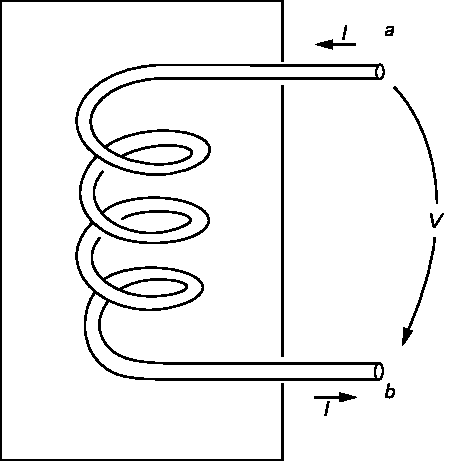
\includegraphics[width=0.5\linewidth]{fyz_fig350.pdf}
    \caption{Induktor
             (\cite[s.~391]{Feynman02})}
    \label{fyz:fig350}
  \end{figure}
   
  \textbf{Indukčnost} se v praxi vytvoří tak, že se navine mnoho závitů drátu do tvaru cívky, 
  přičemž oba konce drátu jsou vyvedeny na svorky umístěné v určité vzdálenosti od cívky (obr. 
  \ref{fyz:fig350}). Přitom je třeba předpokládat, že magnetické pole, vytvořené proudy v cívce, se 
  příliš nerozptyluje do okolního prostoru a neinteraguje s jinými částmi obvodu. Obvykle je toho 
  dosaženo navinutím cívky do tvaru prstence nebo ohraničením magnetického pole navinutím cívky na 
  vhodné železné jádro, nebo konečně uložením cívky do vhodné kovové schránky (schématicky 
  naznačené na obr. \ref{fyz:fig350}). V každém případě počítáme s tím, že ve vnější oblasti blízko 
  svorek \(a\) a \(b\) je magnetické pole zanedbatelné. Dále můžeme předpokládat, že lze zanedbati 
  elektrický náboj, který se v procesu vytváření elektrických polí objevuje na povrchu drátu.
  
  Uplatní-li se všechny tyto aproximace, dostáváme to, co nazveme ideálním induktorem. (Později se 
  vrátíme zpět a budeme hovořit o procesech v reálné cívce.) Tvrdíme, že v případě ideálního 
  induktoru je napětí na svorkách rovno \(L(dI/dt)\). Podíváme se, proč je tomu tak. Když cívkou 
  prochází elektrický proud, vzniká v ní magnetické pole, jehož velikost je přímo úměrná proudu. 
  Mění-li se proud v čase, magnetické pole se mění taktéž. Obecně je \(\rot{E}\) rovna 
  \(-d\vec{B}/dt\) nebo jinak vyjádřeno, křivkový integrál \(\vec{E}\) po kterékoliv uzavřené 
  křivce je rovem záporně vzaté rychlosti změny toku vektoru \(\vec{B}\) plochou smyčky. Uvažujme 
  například následující křivku: začněme na svorce \(a\), postupujme cívkou (přičemž stále zůstáváme 
  uvnitř drátěného vodiče) ke svorce \(b\) a vzduchem ve vnějším prostoru se vraťme na svorku 
  \(a\). Křivkový integrál vektoru \(\vec{E}\) po této uzavřené dráze lze vyjádřit jako součet dvou 
  integrálů
  \begin{equation}\label{fyz:eq468}
   \oint\vec{E}\cdot\dd{s}
     = \limitint_{\mathclap{\substack{a\\\text{cívkou}}}}^{\quad b}\vec{E}\cdot\dd{\vec{s}}
     + \limitint_{\mathclap{\substack{a\\\text{mimo cívku}}}}^{\quad b}\vec{E}\cdot\dd{\vec{s}}.
  \end{equation}
  Jak jsme se přesvědčili už dříve, uvnitř dokonalého vodiče nemohou existovat žádná elektrická 
  pole. (I nejmenší pole by vyvolala nekonečné proudy.) Proto je integrál z \(a\) do \(b\) cívkou 
  roven nule. Celý příspěvek ke křivkovému integrálu \(\vec{E}\) pochází z dráhy vedené mimo cívku 
  od svorky \(b\) ke svorce \(a\). Pokud jsme předpokládali, že v prostoru mimo „schránku“ žádná 
  magnetická pole nejsou, nezávisí tato část integrálu na zvolené dráze a můžeme tedy pro oba 
  výstupy zavést potenciály. Jejich rozdíl je to, co nazýváme napětím \(U\), takže
  \begin{equation}\label{fyz:eq469}
    U = -\int_a^b\vec{E}\cdot\dd{\vec{s}} = - \oint\vec{E}\cdot\dd{\vec{s}}.
  \end{equation}
  Úplný křivkový integrál představuje to, co jsme již dříve nazvali elektromotorickým napětím a je 
  rovem rychlosti změny magnetického indukčního toku v cívce. Taktéž už jsme dříve viděli, že toto 
  elektromotorické napětí je rovno záporně vzaté rychlosti změny elektrického proudu, takže bude
  \begin{equation}\label{fyz:eq470}
    U = -\mathscr{E} = - L\der{I}{t},
  \end{equation}
  kde \(L\) je \textbf{indukčnost cívky}. Pokud \(dI/dt = i\omega I\), dostáváme 
  \begin{equation}\label{fyz:eq471}
    U = i\omega LI.
  \end{equation}
  
  Způsob, jakým jsme popsali ideální indukčnost, ilustruje obecný přístup k obvodu s ideálními 
  prvky obvykle nazývaném \emph{obvod se soustředěnými parametry}. Vlastnosti takových prvků lze 
  úplně popsat pomocí proudů a napětí na jejich svorkách. Udělají-li se vhodné aproximace, je možné 
  upustit ze zřetele velkou složitost polí, vznikajících uvnitř příslušného objektu. To, co se děje 
  uvnitř, je odděleno od toho, co se děje venku.
  
  Pro všechny prvky obvodu najdeme vztahy, připomínající (\ref{fyz:eq471}), v nichž je napětí přímo 
  úměrné proudu, přičemž součinitelem úměrnosti je obecně komplexní číslo. Tento komplexní 
  součinitel se nazývá \textbf{impedance} a obvykle se označuje \(Z\). V obecném případě je funkcí 
  úhlové frekvence \(\omega\). Pro každý ideální prvek tedy můžeme napsat, že
  \begin{equation}\label{fyz:eq472}
    U = \frac{U}{I} = \frac{\hat{U}}{\hat{I}} = Z.
  \end{equation}
  V případě indukčnosti bude
  \begin{equation}\label{fyz:eq473}
    Z(\text{indukčnost}) = Z_L = i\omega L.\footnote{\(Z_L\) nazýváme induktance}
  \end{equation}
  
  \begin{figure}[ht!] %\ref{fyz:fig351}
    \centering
    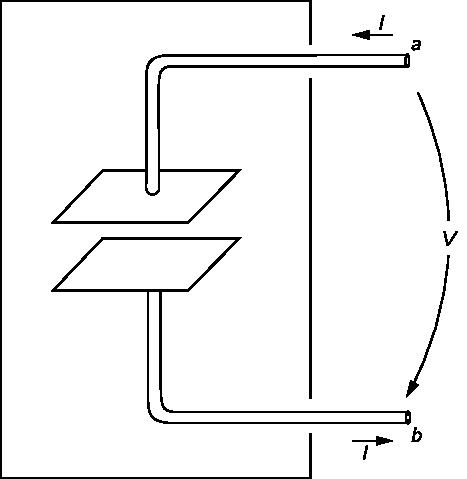
\includegraphics[width=0.5\linewidth]{fyz_fig351.pdf}
    \caption{Kapacitor
             (\cite[s.~392]{Feynman02})}
    \label{fyz:fig351}
  \end{figure}

  Ze stejného hlediska se nyní podívejme na \textbf{kapacitor} (kondenzátor)\footnote{Jsou lidé, 
  kteří říkají, že bychom měli objekty nazývat „induktor“ a „kapacitor" a jejich vlastnosti 
  „indukčnost“a „kapacita“ (podobně jako „rezistor“ a „odpor“). Dáváme přednost používání výrazů, 
  které se používají v laboratoři. Většina lidí stále nazývá „indukčností“ jak skutečnou cívku, tak 
  její indukčnost \(L\).}. Skládá se z páru vodivých elektrod, které jsou dvěma drátěnými vodiči 
  připojeny k vhodným svorkám. Elektrody mohou mít jakýkoliv tvar a často jsou od sebe odděleny 
  nějakou dielektrickou látkou. Schématicky je toto uspořádání znázorněno na obr. \ref{fyz:fig351}. 
  Opět uděláme několik zjednodušujících předpokladů

  Elektrody a přívodné dráty budeme pokládat za dokonalé vodiče. Budeme také počítat s tím, že mezi 
  elektrodami je dokonalá izolace, takže jí nemohou z jedné elektrody na druhou procházet žádné 
  náboje. Dále předpokládáme, že oba vodiče představující elektrody kondenzátoru jsou blízko sebe, 
  ale daleko od jiných vodičů a tedy všechny siločáry, které vycházejí z jedné elektrody, končí v 
  druhé elektrodě. Pak na elektrodách vždy existují stejně velké náboje opačného znaménka a tyto 
  náboje jsou mnohem větší než náboje na površích přívodních vodičů. Nakonec budeme předpokládat, 
  že v blízkosti kondenzátoru nejsou žádná magnetická pole. 
  
  Nyní uvažujme křivkový integrál z \(\vec{E}\) po uzavřené dráze, která začíná na svorce \(a\), 
  jde po drátu k vrchní elektrodě kondenzátoru, prochází mezerou mezi elektrodami na spodní z nich 
  a od něj po přívodním drátu ke svorce \(b\), od něhož se vrací prostorem mimo kondenzátor ke 
  svorce \(a\). Protože tam není žádné magnetické pole, křivkový integrál \(\vec{E}\) po této 
  uzavřené dráze je roven nule. Lze jej rozdělit na tři složky:
  \begin{equation}\label{fyz:eq474}
   \oint\vec{E}\cdot\dd{s}
     = \limitint_{\mathclap{\substack{\\\text{vodiči}}}}\vec{E}\cdot\dd{\vec{s}}
     + \limitint_{\mathclap{\substack{\text{mezi}\\\text{elektrodami}}}}\vec{E}\cdot\dd{\vec{s}}
     + \limitint_{\mathclap{\substack{a\\\text{venku}}}}^{\quad b}\vec{E}\cdot\dd{\vec{s}}.
  \end{equation}
  
  Integrál po přívodních vodičích je roven nule, neboť uvnitř dokonalých vodičů žádná elektrická 
  pole nejsou. Integrál z \(b\) do \(a\) po dráze vedoucí mimo kondenzátor je roven záporně vzatému 
  rozdílu potenciálů mezi oběma svorkami. A protože jsme předpokládali, že elektrody jsou nějakým 
  způsobem odizolovány od okolního světa, musí být celkový náboj na nich roven nule. Je-li na horní 
  elektrodě náboj \(Q\) na spodní se nachází stejně velký náboj s opačným znaménkem, tj. \(-Q\). 
  Předtím jsme se dozvěděli, že mají-li dva vodiče stejně velké náboje s opačnými znaménky, plus a 
  minus \(Q\) je mezi nimi rozdíl potenciálů \(Q/C\), kde \(C\) je vzájemná kapacita obou vodičů. Z 
  rovnosti (\ref{fyz:eq474}) vyplývá, že rozdíl potenciálů mezi svorkami \(a\) a \(b\) je roven 
  rozdílu potenciálů mezi elektrodami. Dostáváme proto výsledek, že
  \begin{equation*}
    U = \frac{Q}{C}.
  \end{equation*}
  
  Elektrický proud \(I\) vstupující do kondenzátoru svorkou \(a\) (a vystupující svorkou \(b\)) je 
  roven \(dQ/dt\), tj. rychlosti změny elektrického náboje na elektrodách. Zapíšeme-li \(dU/dt\) 
  jako \(i\omega U\), můžeme vztah mezi napětím a proudem pro kondenzátor vyjádřit v následujícím 
  tvaru:
  \begin{equation*}
    i\omega U = \frac{I}{C}
  \end{equation*}
  resp.
  \begin{equation}\label{fyz:eq475}
    U = \frac{I}{i\omega C}.
  \end{equation}
  Impedance \(Z\) idealizovaného kondenzátoru je tedy rovna 
  \begin{equation}\label{fyz:eq476}
    Z(\text{kapacita}) = Z_C = \frac{1}{i\omega C}.\footnote{\(Z_C\) nazýváme kapacitance}
  \end{equation}

  Třetí prvek, který potřebujeme prozkoumat, je \textbf{rezistor}. Protože jsme se však dosud 
  nezabývali elektrickými vlastnosti reálných látek, nejsme ještě připraveni hovořit o procesech, k 
  nimž dochází uvnitř reálného vodiče. Budeme pouze muset přijmout fakt, že uvnitř reálných látek 
  mohou existovat elektrická pole, že tato elektrická pole mohou vyvolat tok elektrického náboje, 
  tj. elektrický proud a že tento proud je přímo úměrný integrálu elektrického pole od jednoho 
  konce vodiče k druhému. Představujeme si přitom, že ideální rezistor je konstruován tak, jak 
  ukazuje obr. \ref{fyz:fig352}. Od svorek \(a\) a \(b\) vedou k oběma koncům tyče z odporového 
  materiálu dva přívodní dráty, které pokládáme za dokonalé vodiče. Obvyklou posloupností úvah 
  dospějeme k výsledku, že rozdíl potenciálů mezi svorkami \(a\) a \(b\) je roven křivkovému 
  integrálu vnějšího elektrického pole, který je též rovem křivkovému integrálu elektrického pole 
  podél tyče z odporového materiálu.
  
  \begin{figure}[ht!] %\ref{fyz:fig352}
    \centering
    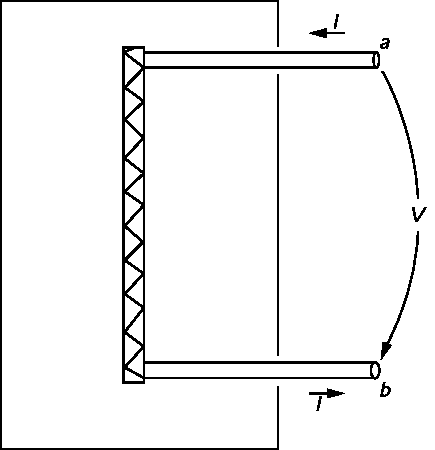
\includegraphics[width=0.5\linewidth]{fyz_fig352.pdf}
    \caption{Rezistor
             (\cite[s.~394]{Feynman02})}
    \label{fyz:fig352}
  \end{figure}
  
  Z toho pak vyplývá, že proud \(I\) rezistorem je přímo úměrný napětí \(U\) na výstupech:
  \begin{equation*}
    I = \frac{U}{R},
  \end{equation*}
  kde se \(R\) nazývá \textbf{odpor} (\emph{rezistance}). Později uvidíme, že vztah mezi proudem a 
  napětím je pouze přibližně lineární. Také uvidíme, že tuto přibližnou přímou úměrnost lze 
  pokládat za nezávislou na frekvenci změny proudu a napětí pouze tehdy, když tato frekvence není 
  příliš vysoká. Při střídavých proudech je v tomto případě napětí na odporu ve fázi s proudem, což 
  znamená, že impedance je reálným číslem:
  \begin{equation}\label{fyz:eq477}
    Z(\text{odpor}) = Z_R = R.
  \end{equation}
  
  Výsledky, které jsme dostali pro tři reálné prvky obvodů - \emph{induktor}, \emph{kapacitor} a 
  \emph{rezistor} - jsou shrnuty na obr. \ref{fyz:fig353}. Na tomto, jakož i na předcházejících 
  obrázcích, jsme vyznačili napětí šipkou, která směřuje od jednoho výstupu k druhému.

  \begin{figure}[hb!] %\ref{fyz:fig353}
    \centering
    \begin{tabular}{cccc}
     \subfloat[ ]{\label{fyz:fig353a}
       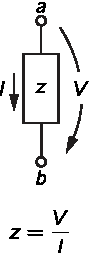
\includegraphics[width=0.2\linewidth]{fyz_fig353a.pdf}}
     \subfloat[ ]{\label{fyz:fig353b}
       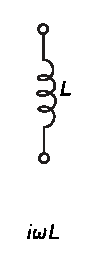
\includegraphics[width=0.2\linewidth]{fyz_fig353b.pdf}}
     \subfloat[ ]{\label{fyz:fig353c}
       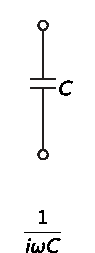
\includegraphics[width=0.2\linewidth]{fyz_fig353c.pdf}}
     \subfloat[ ]{\label{fyz:fig353d}
       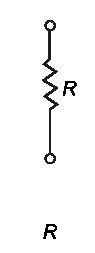
\includegraphics[width=0.2\linewidth]{fyz_fig353d.pdf}}
    \end{tabular}
    \caption{Ideální (pasivní) prvky obvodu se soustředěnými parametry
             (\cite[s.~394]{Feynman02}).}
    \label{fyz:fig353}
  \end{figure}
  
  Je-li napětí „kladné“, tj. má-li svorka \(a\) vyšší potenciál než svorka \(b\), ukazuje šipka 
  směr kladného „úbytku potenciálu“.
  
  Ačkoliv nyní probíráme střídavé proudy, můžeme sem zahrnout i obvody s ustálenými proudy, a to 
  tím, že provedeme limitu pro případ, že se frekvence \(\omega\) blíží nule. Při nulové frekvenci, 
  tj. pro stejnosměrný proud, klesá impedance indukčnosti k nule - cívka představuje spojení 
  nakrátko. Impedance kapacity pro stejnosměrný proud roste do nekonečna - kondenzátor představuje 
  přerušení obvodu. Protože impedance odporu nezávisí na frekvenci, je rezistor jediným prvkem, 
  který zůstává i při analýze obvodů se stejnosměrným proudem.
  
  V těchto prvcích elektrických obvodů, které jsme dosud popsali, jsou proud a napětí navzájem 
  úměrné veličiny. Je-li jedna z nich rovna nule, je rovna nule i druhá. Obvykle chápeme tyto věci 
  takto: přiložené napětí je „příčinou“ proudu, nebo proud „způsobuje vznik“ napětí na výstupech - 
  tedy uvedené prvky v určitém smyslu reagují na vnucené vnější podmínky. Proto takovéto prvky 
  nazýváme prvky \textbf{pasivní}. Z tohoto aspektu jsou protikladem \textbf{aktivních} prvků, 
  takových jako jsou generátory, probírané v následujícím článku, které jsou zdroji kmitavých 
  proudů a napětí v elektrickém obvodu.
  \newpage
\section{Generátory}\label{fyz:IIchapXXIIsecII}
  Nyní je třeba pohovořit o \emph{aktivním prvku elektrických obvodů}, tj. o tom prvku, který je 
  zdrojem proudů a napětí v obvodu - o \textbf{generátoru}.
  
  \begin{figure}[ht!] %\ref{fyz:fig354}
    \centering
    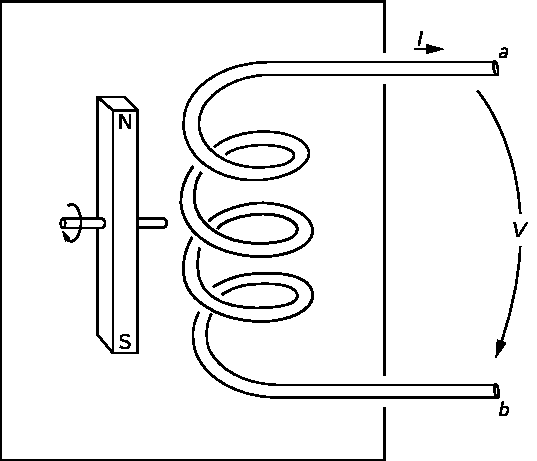
\includegraphics[width=0.7\linewidth]{fyz_fig354.pdf}
    \caption{Generátor skládající se z pevné cívky a rotujícího magnetického pole
             (\cite[s.~395]{Feynman02})}
    \label{fyz:fig354}
  \end{figure}
  
  Mějme cívku podobnou té, o níž jsme hovořili v souvislosti s indukčností, pouze s tím rozdílem, 
  že má velmi malý počet závitů, takže magnetické pole jí procházejícího proudu lze zanedbat. Nechť 
  se tato cívka nachází v proměnném magnetickém poli, například v takovém, jaké by vytvářel 
  otáčející se magnet (obr. \ref{fyz:fig354}). (Dřív jsme ukázali, že pole takového rotujícího 
  magnetu lze vytvořit i vhodnou soustavou cívek napájených střídavým proudem.) Opět musíme provést 
  několik zjednodušujících předpokladů. Jde o všechny ty předpoklady, které jsme popsali v případě 
  idealizované cívky. Jmenovitě budeme předpokládat, že proměnné magnetické pole je omezeno na 
  určitou oblast v blízkosti cívky a mimo generátor se v prostoru mezi svorkami neobjevuje.

  \begin{figure}[ht!] %\ref{fyz:fig355}
    \centering
    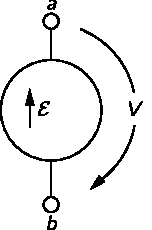
\includegraphics[width=0.2\linewidth]{fyz_fig355.pdf}
    \caption{Značka ideálního generátoru
             (\cite[s.~396]{Feynman02})}
    \label{fyz:fig355}
  \end{figure}
  
  Přesně tak jako při analýze indukčnosti uvažujeme křivkový integrál \(\vec{E}\) podél uzavřené 
  smyčky, která začíná na svorce \(a\), prochází cívkou ke svorce \(b\) a prostorem mezi oběma 
  cívkami se vrací do svého východiska. Znovu dospějeme k závěru, že rozdíl mezi výstupy je roven 
  křivkovému integrálu \(\vec{E}\) po této uzavřené křivce:
  \begin{equation}\label{fyz:eq478}
   U = -\oint\vec{E}\cdot\dd{s}.
  \end{equation}

  Tento křivkový integrál představuje elektromotorické napětí v obvodu. Proto rozdíl potenciálů 
  \(U\) na výstupech generátoru je také roven rychlosti změny magnetického indukčního toku cívkou, 
  vynásobenému počtem závitů:
  \begin{equation}\label{fyz:eq479}
   U = -\mathscr{E} = \der{ }{t}(\text{tok}).
  \end{equation}
  V případě ideálního generátoru předpokládáme, že magnetický tok procházející cívkou je určen 
  pouze vnějšími podmínkami (takovými jako například úhlová rychlost rotujícího magnetického pole) 
  a není vůbec ovlivněn proudem procházejícím generátorem. Z toho důvodu generátor - alespoň 
  ideální generátor, o němž zde hovoříme - nemá žádnou impedanci. Rozdíl potenciálů na jeho 
  svorkách určuje elektromotorické napětí \(\mathscr{E}(t)\), které se generátoru libovolně 
  přiřadilo. Takový ideální generátor budeme zakreslovat značkou ukázanou na obr. \ref{fyz:fig355}. 
  Malá šipka ukazuje směr kladného elektromotorického napětí. V generátoru zobrazeném na obr. 
  \ref{fyz:fig355} bude kladné elektromotorické napětí vytvářet napětí \(U=\mathscr{E}\), přičemž 
  svorka \(a\) bude mít vyšší potenciál než Svorka \(b\).
  
  Existuje i jiný způsob, jak sestrojit generátor. Ten pak bude úplně jiný, pokud se jedná o 
  vnitřní uspořádání, ale naprosto nerozlišitelný od výše popsaného z hlediska toho, co se děje za 
  jeho svorkami. Představuje cívku se závity drátu, která se otáčí ve stálém magnetickém poli tak, 
  jak je to vyznačeno na obr. \ref{fyz:fig356}. Abychom zvýraznili existenci magnetického pole, je 
  tam vyobrazen tyčový magnet. Je pravda, že by se mohl nahradit jakýmkoliv jiným zdrojem 
  magnetického pole, například další cívkou napájenou ustáleným elektrickým proudem. Jak je vidět z 
  obrázku, rotující cívka je spojena s vnějším světem pomocí kluzných kontaktů nebo „sběracích 
  kroužků“. Opět nás zajímá, jaký rozdíl potenciálů vzniká mezi oběma svorkami \(a\) a \(b\). Je 
  roven integrálu intenzity elektrického pole po dráze vedené mimo generátor od svorky \(a\) k 
  svorce \(b\).

  \begin{figure}[ht!] %\ref{fyz:fig356}
    \centering
    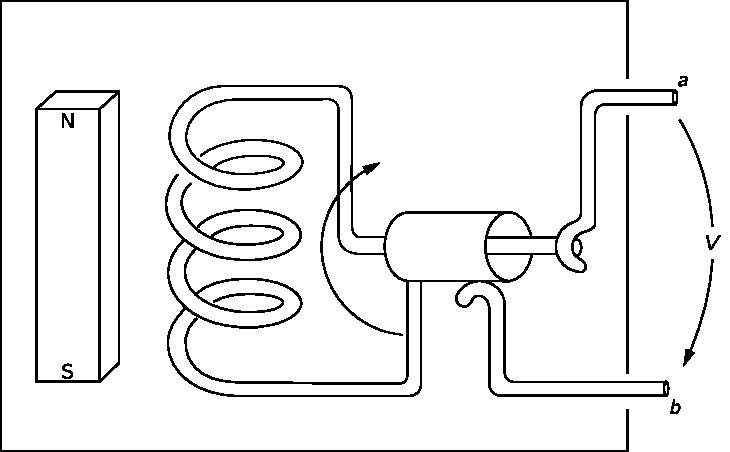
\includegraphics[width=0.7\linewidth]{fyz_fig356.pdf}
    \caption{Generátor skládající se z cívky rotující v konstantním magnetickém poli
             (\cite[s.~397]{Feynman02})}
    \label{fyz:fig356}
  \end{figure}
  
  V systému znázorněném na obr. \ref{fyz:fig356} nyní nejsou žádná proměnná magnetická pole. Na 
  první pohled bychom se proto mohli podivit, jak se vůbec může objevit nějaké napětí na svorkách 
  generátoru. Vlastně nikde v něm nejsou ani žádná elektrická pole. Jako obyčejně pro naše ideální 
  prvky, i zde předpokládáme, že vodiče uvnitř generátoru jsou z dokonale vodivého materiálu a jak 
  jsme řekli mnohokrát, uvnitř dokonalého vodiče je elektrické pole rovno nule. Ale to není pravda. 
  Totiž pravda to není tehdy, když se vodič pohybuje v magnetickém poli. Správným tvrzením je, že 
  uvnitř dokonalého vodiče musí být rovna nule výsledná síla působící na každý náboj. V opačném 
  případě by došlo k nekonečně velkému toku volných nábojů.
  
  Vždy však platí, že součet elektrického pole \(\vec{E}\) a vektorového součinu rychlosti vodiče a 
  magnetického pole \(\vec{B}\), což mimochodem představuje celkovou sílu, která by působila na 
  jednotkový náboj, musí mít uvnitř vodiče nulovou hodnotu:
  \begin{equation}\label{fyz:eq480}
   \vec{F}/\text{náboj} = \vec{E} + \vec{v}\times\vec{B} = 0\qquad(\text{v dokonalém vodiči}).
  \end{equation}
  (\(\vec{v}\) je zde rychlost vodiče). Naše pozdější tvrzení, že uvnitř dokonalého vodiče nejsou 
  elektrická pole je v pořádku, je-li rychlost vodiče v rovna nule; jinak správné tvrzení 
  představuje rovnice (\ref{fyz:eq480}). Vraťme se k našemu generátoru, jehož schéma je na obr. 
  \ref{fyz:fig356}. Nyní vidíme, že křivkový integrál elektrického pole \(\vec{E}\) od svorky \(a\) 
  po svorku \(b\) po dráze vedoucí vodiči v generátoru musí být roven křivkovému integrálu součinu 
  \(\vec{v}\times\vec{B}\) počítanému po téže dráze, tj.
  \begin{equation}\label{fyz:eq481}
       \limitint_{\mathclap{\substack{a\\\text{uvnitř vodiče}}}}^{\quad b}\vec{E}\cdot\dd{\vec{s}} =
     - \limitint_{\mathclap{\substack{a\\\text{uvnitř vodiče}}}}^{\quad b} 
                                   (\vec{v}\times\vec{B})\cdot\dd{\vec{s}}.
  \end{equation}

  Stále však platí, že křivkový integrál \(\vec{E}\) po úplně uzavřené dráze, včetně návratu od 
  \(b\) k \(a\) prostorem mimo generátor, musí být roven nule, neboť tam nejsou proměnná magnetická 
  pole. Proto je první integrál v rovnici (\ref{fyz:eq481}) roven i napětí \(U\) mezi oběma 
  svorkami. Ukazuje se, že integrál na pravé straně (\ref{fyz:eq481}) je právě roven rychlosti 
  změny součinu magnetického indukčního toku cívkou a počtu jejích závitů a podle pravidla o toku 
  je proto roven elektromotorickému napětí v cívce. Tak opět docházíme k výsledku, že rozdíl 
  potenciálů svorek je roven záporně vzatému elektromotorickému napětí v obvodu, což souhlasí se 
  vztahem (\ref{fyz:eq479}). Máme-li tedy nějaký generátor, v němž se magnetické pole v blízkosti 
  nepohybující se cívky mění, nebo takový, v němž se cívka pohybuje ve stálém magnetickém poli, 
  jsou vnější vlastnosti generátorů tytéž. Na svorkách generátoru existuje napětí \(U\), jež 
  nezávisí na proudu v obvodu, ale jen na podmínkách uvnitř generátoru a tyto nastavujeme podle 
  naší libovůle. 
  
  Pokud se snažíme pochopit činnost generátorů z hlediska Maxwellových rovnic, mohli bychom se také 
  zeptat, jak je to v případě obyčejného \textbf{galvanického článku}, například takového, který se 
  používá do baterky. Jde taktéž o generátor, tj. zdroj napětí, ačkoliv se, samozřejmě, vyskytuje 
  pouze v obvodech se stejnosměrným proudem. Obr. \ref{fyz:fig357} ukazuje druh článku, který je 
  pro porozumění nejednodušší. Představme si dvě kovové destičky ponořené do nějakého chemického 
  roztoku. Předpokládejme, že roztok obsahuje kladné a záporné ionty. Nechť jedny ionty, řekněme 
  záporné, jsou mnohem těžší než ionty opačné polarity, takže jejich difuzní pohyb v roztoku je 
  mnohem pomalejší. Nakonec budeme předpokládat, že se nějakým způsobem zabezpečilo, aby se 
  koncentrace roztoku od místa k místu v kapalině měnila tak, že počet iontů obou polarit je 
  řekněme u spodní destičky mnohem větší než koncentrace iontů v blízkosti horní destičky, V 
  důsledku své velké pohyblivosti se kladné ionty budou pohotověji přesouvat do oblasti s nižší 
  koncentrací, takže množství kladného náboje přicházející k horní destičce bude trochu převyšovat 
  množství záporného náboje, jež tam také dospěje.

  \begin{figure}[ht!] %\ref{fyz:fig357}
    \centering
    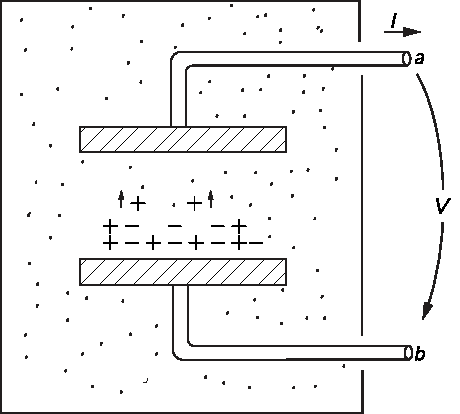
\includegraphics[width=0.7\linewidth]{fyz_fig357.pdf}
    \caption{Galvanický článek
             (\cite[s.~398]{Feynman02})}
    \label{fyz:fig357}
  \end{figure}
  
  Horní destička se proto bude nabíjet kladně a výsledný náboj spodní destičky bude záporný. Podle 
  toho, jak k horní destičce difunduje víc a víc nábojů, bude potenciál této destičky růst, až se 
  mezi destičkami vytvoří takové elektrické pole, které svým silovým účinkem na ionty přesně 
  vykompenzuje jejich nadměrnou pohyblivost. V důsledku toho získají obě destičky rychle takový 
  rozdíl potenciálů, který charakterizuje vnitřní stavbu článku.
  
  Stejnými úvahami jako v případě ideálního kondenzátoru se přesvědčíme, že není-li už žádná 
  výsledná difuze iontů, je rozdíl potenciálů mezi svorkami \(a\) a \(b\) přesně rovem křivkovému 
  integrálu elektrického pole mezi oběma destičkami. Je pravda, že mezi kondenzátorem a takovým 
  galvanickým článkem je podstatný rozdíl. Spojíme-li na okamžik svorky kondenzátoru nakrátko, 
  kondenzátor se vybije a na svorkách už žádné napětí nebude. V případě galvanického článku lze 
  proud ze svorek odebírat neustále bez jakékoliv změny elektromotorického napětí - dokud, 
  přirozeně, nebudou příslušné chemikálie spotřebovány. V reálném článku je pozorováno, že 
  stoupá-li z něj odebíraný proud, napětí na jeho svorkách se snižuje. Avšak v rámci výše 
  provedených abstrakcí si můžeme představit takový ideální článek, v němž napětí na svorkách 
  nezávisí na proudu. Na reálný článek se pak můžeme dívat jako na ideální článek spojený do série 
  s rezistorem.
  
\section{Sítě s ideálnímy prvky. Kirchhoffova pravidla}\label{fyz:IIchapXXIIsecIII}
  Zajímáme-li se jen o to, co se děje mimo prvek, je popis ideálních prvků obvodů - jak už jsme 
  viděli - docela jednoduchý. Proud a napětí souvisí lineárně. Ale procesy, které uvnitř toho 
  kterého prvku skutečně probíhají, jsou značně komplikované a podat jejich přesný popis z hlediska 
  Maxwellových rovnic je velmi obtížné. Představme si pokus přesně popsat elektrická a magnetická 
  pole uvnitř rádia, obsahujícího stovky odporů, kondenzátorů a cívek. Analyzovat takovou věc 
  pomocí Maxwellových rovnic by byla prakticky nesplnitelná úloha. Provedeme-li však mnohé 
  aproximace, které jsme uvedli v článku \ref{fyz:IIchapXXIIsecII} a podstatné charakteristiky 
  reálných prvků elektrických obvodů sumarizujeme ve formě jejich idealizací, získáváme možnost 
  analyzovat elektrický obvod poměrně jednoduchým způsobem. Nyní ukážeme, jak se to dělá.
  
  \begin{figure}[ht!] %\ref{fyz:fig358}
    \centering
    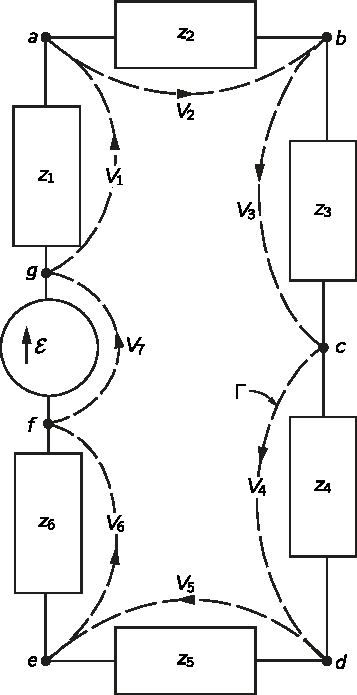
\includegraphics[width=0.5\linewidth]{fyz_fig358.pdf}
    \caption{Součet úbytků napětí po každé uzavřené dráze je roven nule
             (\cite[s.~399]{Feynman02})}
    \label{fyz:fig358}
  \end{figure}
  
  Mějme obvod skládající se z generátoru a několika impedancí propojených tak, jak to ukazuje obr. 
  \ref{fyz:fig358}. V prostoru mimo samotné prvky obvodu není souhlasně s našimi aproximacemi žádné 
  magnetické pole. Proto je křivkový integrál \(\vec{E}\) pokaždé dráze neprocházející ani jedním z 
  prvků roven nule. Nyní prozkoumejme křivku \(\Gamma\), která vede kolem našeho obvodu a je na 
  obr. \ref{fyz:fig358} vykreslena čárkovaně. Křivkový integrál \(\vec{E}\) po této křivce se 
  skládá z několika příspěvků, z nichž každý je křivkovým integrálem počítaným po dráze jdoucí od 
  jedné svorky nějakého prvku k další jeho svorce. Tento křivkový integrál jsme nazvali 
  \emph{úbytkem napětí} na příslušném prvku.
  
  Úplný křivkový integrál je pak přesně roven součtu úbytků napětí na všech prvcích obvodu: 
  \begin{equation}\label{fyz:eq482}
    \oint\vec{E}\cdot\dd{s} = \sum U_n.
  \end{equation}
  Je-li tento křivkový integrál rovem nule, platí, že součet rozdílů potenciálů podél uzavřeného 
  elektrického obvodu je roven nule:
  \begin{equation}\label{fyz:eq483}
    \sum_{\mathclap{\substack{\text{podél}\\\text{každéhé}\\\text{uzavřeného}\\\text{obvodu}}}} 
         U_n = 0.
  \end{equation}
  Tento výsledek vyplývá z jedné z Maxwellových rovnic, podle níž v oblasti, kde nejsou magnetická 
  pole, je křivkový integrál z \(\vec{E}\) po každé uzavřené křivce roven nule. 
  
  Nyní prozkoumejme takový obvod, jako je na obr. \ref{fyz:fig359}. Vodorovná čára spojující svorky 
  \(a\), \(b\), \(c\) a \(d\) má označovat, že všechny tyto svorky jsou spolu spojeny nebo že jsou 
  propojeny spojovacími vodiči se zanedbatelným odporem. V každém případě podle tohoto schématu 
  mají svorky \(a\), \(b\), \(c\) a \(d\) stejný potenciál a podobně svorky \(e\), \(f\), \(g\) a 
  \(h\) jsou také všechny na témže společném potenciálu. Pak je na každém z těchto čtyř prvků 
  stejný úbytek napětí \(U\).

  \begin{figure}[ht!] %\ref{fyz:fig359}
    \centering
    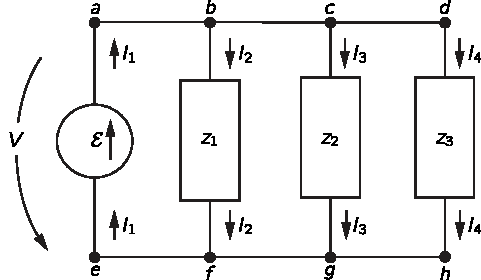
\includegraphics[width=0.5\linewidth]{fyz_fig359.pdf}
    \caption{Algebraický součet proudů vstupujících do každého uzlu je roven nule
             (\cite[s.~400]{Feynman02})}
    \label{fyz:fig359}
  \end{figure}
  
  Jedna z našich idealizací spočívala v tom, že na svorkách impedancí se akumulují pouze 
  zanedbatelné elektrické náboje. Nyní uděláme předpoklad, že lze zanedbat i jakékoliv elektrické 
  náboje sídlící na vodičích spojujících mezi sebou svorky. Zákon zachování elektrického náboje pak 
  vyžaduje, aby každý náboj, který vychází z jednoho prvku našeho obvodu ihned vstoupil do nějakého 
  jiného prvku. Nebo - což je totéž - požadujeme, aby algebraický součet proudů přicházejících do 
  jakéhokoliv daného spojovacího bodu byl roven nule. Spojovacím bodem rozumíme, samozřejmě, 
  jakoukoliv množinu svorek (takových jako \(a\), \(b\), \(c\) a \(d\) na obr. \ref{fyz:fig359}), 
  které jsou spolu propojeny. Taková množina propojených svorek se obvykle nazývá \emph{„uzel“}. 
  Zákon zachování náboje pak vyžaduje, aby pro obvod na obr. \ref{fyz:fig359} platilo
  \begin{equation}\label{fyz:eq484}
    I_1 - I_2 - I_3 - I_4 = 0.
  \end{equation}
  Součet proudů vstupujících do uzlu, který se skládá ze čtyř svorek \(e\), \(j\), \(g\) a \(h\), 
  musí být také roven nule:
  \begin{equation}\label{fyz:eq485}
    - I_1 + I_2 + I_3 + I_4 = 0.
  \end{equation}
  Je to ovšem táž rovnice jako (\ref{fyz:eq484}). Tyto rovnice nejsou nezávislé. Obecné pravidlo 
  zní, že součet proudů vstupujících do každého uzlu musí být roven nule.
  \begin{equation}\label{fyz:eq486}
    \sum_{\mathclap{\substack{\text{do}\\\text{uzlu}}}} I_n = 0.
  \end{equation}
  
  Náš dřívější závěr o tom, že součet úbytků napětí v uzavřeném obvodu je roven nule, musí ve 
  složité síti platit pro každý uzavřený obvod. Kromě toho pro každý uzel musí platit náš výsledek, 
  že algebraický součet proudů vstupujících do uzlu je roven nule. Tyto dvě rovnice jsou známy jako 
  \textbf{Kirchhoffova pravidla}. Jejich pomocí lze najít proudy a napětí v jakékoliv síti.
  
  \begin{figure}[ht!] %\ref{fyz:fig360}
    \centering
    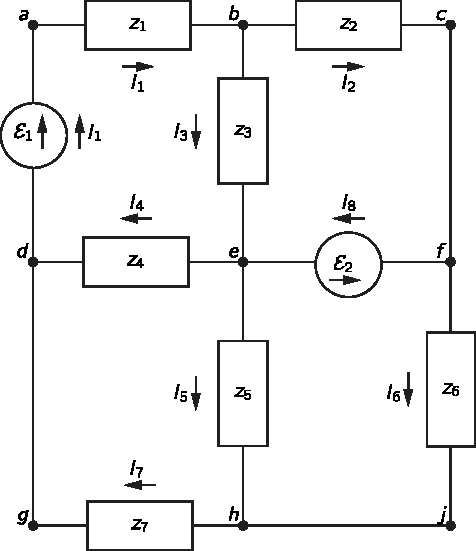
\includegraphics[width=0.7\linewidth]{fyz_fig360.pdf}
    \caption{Analýza sítě pomocí Kirchhoffových pravidel
             (\cite[s.~401]{Feynman02})}
    \label{fyz:fig360}
  \end{figure}
  
  Uvažujme složitější obvod, jehož schéma je na obr. \ref{fyz:fig360}. Jak najdeme proudy a napětí 
  v tomto obvodu? Lze je určit následujícím prostým způsobem. Odděleně prozkoumáme každý ze čtyř 
  uzavřených obvodů vyskytující se v tomto obvodu. (Například jeden obvod vede od svorky \(a\) ke 
  svorce \(b\) a dále přes svorky \(e\) a \(d\) zpět ke svorce \(a\).) Pro každý z nich napíšeme 
  rovnici vyjadřující první z Kirchhoffových zákonů - že součet všech napětí podél obvodu je roven 
  nule.
  
  Je nutné pamatovat na to, aby se úbytek napětí počítal jako kladný, postupujeme-li ve směru 
  proudu, a jako záporný, procházíme-li v opačném směru než proud. Musíme také mít na zřeteli, že 
  úbytek napětí na generátoru je roven záporné hodnotě elektromotorického napětí v příslušném 
  směru. Pro jednoduchý obvod, který začíná a končí na svorce \(a\) dostaneme rovnici
  \begin{equation*}
    z_1I_1 + Z_3I_3 + Z_4I_4 -\mathscr{E}_1 = 0.
  \end{equation*}
  Použitím stejného pravidla na zbývající obvody bychom dostali další tři rovnice téhož druhu. 
  
  Dále je třeba napsat rovnici pro proud, a to pro každý uzel v našem schématu. Například sečtení 
  proudů přitékajících do uzlu u svorky \(b\) vede k rovnici
  \begin{equation*}
    I_1 - I_3 - I_2 = 0.
  \end{equation*}
  Analogicky by rovnice pro proudy v případě uzlu označeného \(e\) vypadala takto:
  \begin{equation*}
    I_3 - I_4 + I_8 - I_5 = 0.
  \end{equation*}
  Pro dané schéma existuje pět takovýchto rovnic pro proudy. Ukazuje se však, že kteroukoliv z 
  těchto rovnic lze odvodit ze zbývajících čtyř. Existují proto jen čtyři nezávislé rovnice pro 
  proudy. Máme tedy celkem osm \emph{nezávislých lineárních rovnic} - čtyři rovnice pro napětí 
  a čtyři pro proudy. Z těchto osmi rovnic lze vypočítat osm neznámých proudů. Budeme-li tyto 
  proudy znát, bude obvod vyřešen. Úbytek napětí na každém prvku je dán součinem proudu tímto 
  prvkem a jeho impedancí (nebo - jako v případě zdrojů napětí - je už znám). 
  
  Viděli jsme, že při sestavování rovnic pro proudy jsme dostali jednu rovnici, která nebyla 
  nezávislá na jiných. Obecně lze napsat příliš mnoho rovnici pro napětí. Ačkoliv jsme například v 
  případě schématu z obr. \ref{fyz:fig360} uvažovali pouze o čtveřici malých uzavřených obvodů, 
  existuje tam mnoho dalších obvodů, pro něž bychom mohli psát rovnici pro napětí. Je to například 
  uzavřený obvod procházející body \(a\) \(b\) \(c\) \(f\) \(e\) \(d\) \(a\). Jiný obvod sleduje 
  dráhu \(a\) \(b\) \(c\) \(e\) \(h\) \(g\) \(d\) \(a\). Můžete se přesvědčit, že takových obvodů 
  existuje mnoho. Při analýze složitých zapojení se velmi snadno dostane příliš mnoho rovnic. Na 
  to, jak postupovat, aby se napsal pouze minimální počet rovnic, existují pravidla. Ale obvykle už 
  po chvíli přemýšlení lze pochopit, jak dostat správný počet rovnic v nejjednodušším tvaru. Kromě 
  toho napsání jedné - dvou přebytečných rovnic ničemu neublíží. Nepovedou k žádným nesprávným 
  výsledkům, jen k troše zbytečné algebry.
   
  V kapitole \ref{fyz:IchapXXV} dílu \ref{part:FYZI} jsme ukázali, že jsou-li dvě impedance \(Z_1\) 
  a \(Z_2\). zapojeny do \emph{série}, jsou rovnocenné jedné impedanci \(Z_S\) dané vztahem
  \begin{equation}\label{fyz:eq487}
    Z_S = Z_1 + Z_2.
  \end{equation}
  Ukázali jsme také, že jsou-li tyto dvě impedance zapojeny paralelně, jsou rovnocenné jedné 
  impedanci \(Z_P\), dané vztahem
  \begin{equation}\label{fyz:eq488}
    Z_P = \dfrac{1}{\dfrac{1}{Z_1} + \dfrac{1}{Z_2}} = \frac{Z_1Z_2}{Z_1 + Z_2}.
  \end{equation}
  
  \begin{figure}[ht!] %\ref{fyz:fig361}
    \centering
    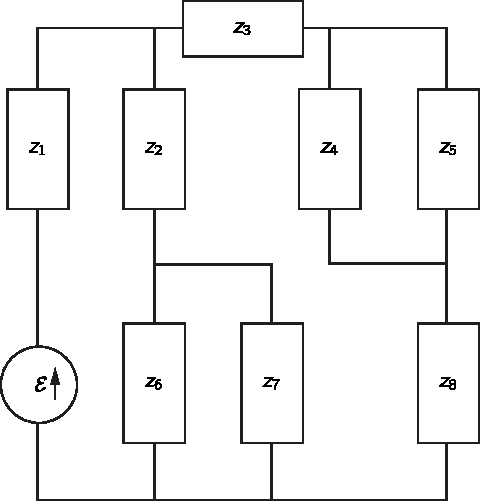
\includegraphics[width=0.7\linewidth]{fyz_fig361.pdf}
    \caption{Obvod, který lze analyzovat pomocí pravidel pro sériové a paralelní zapojení
             (\cite[s.~402]{Feynman02})}
    \label{fyz:fig361}
  \end{figure}
  
  Podíváme-li se zpět, uvidíme, že při odvozování těchto výsledků jsme vlastně použili Kirchhoffovy 
  zákony. Složitá schémata lze často analyzovat opakovaným použitím těchto vzorců pro sériové a 
  paralelní zapojení impedancí. Tímto způsobem lze například analyzovat síť, jejíž schéma je na 
  obr. \ref{fyz:fig361}. Především lze impedance \(Z_4\), a \(Z_5\) jakož i impedance \(Z_6\) a 
  \(Z_7\), nahradit ekvivalenty jejich paralelnímu zapojení. Nato lze impedanci \(Z_2\), kombinovat 
  podle pravidla pro sériové zapojení s ekvivalentem paralelního zapojení \(Z_6\) a \(Z_7\). 
  Pokračuje-li se takto dále, lze celý obvod zredukovat na generátor \(\mathscr{E}\) zapojený do 
  série s jedinou impedancí \(Z\) Proud celým generátorem je pak roven \(\mathscr{E}/Z\). Zpětným 
  postupem lze vypočítat proudy pro každou impedanci.

  \begin{figure}[ht!] %\ref{fyz:fig362}
    \centering
    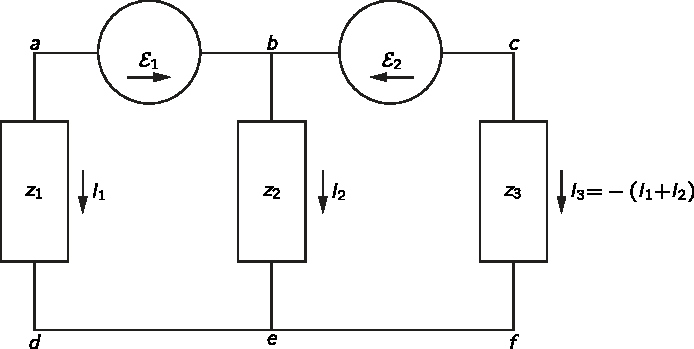
\includegraphics[width=0.8\linewidth]{fyz_fig362.pdf}
    \caption{Obvod, který nelze analyzovat na základě pravidel pro sériové a paralelní zapojení
             (\cite[s.~403]{Feynman02})}
    \label{fyz:fig362}
  \end{figure}
   
  Existují však i taková, a přitom docela jednoduchá zapojení, která nelze touto metodou 
  analyzovat, například schéma na obr. \ref{fyz:fig362}. Při analýze tohoto schématu musíme napsat 
  rovnice pro proudy a pro napětí podle Kirchhoffových pravidel. Udělejme to. Pro proudy existuje 
  jediná rovnice:
  \begin{equation*}
    I_1 + I_2 + I_3 = 0.
  \end{equation*}
  takže ihned víme, že
  \begin{equation*}
    I_1 = - (I_2 + I_3).
  \end{equation*}
  Trochu algebraické práce si můžeme ušetřit tím, že tento výsledek ihned využijeme při psaní 
  rovnic pro napětí. Pro naše schéma existují dvě takové nezávislé rovnice, jsou to
  \begin{align*}
   -\mathscr{E}_1 + I_2Z_2 - I_1Z_1         &= 0 \\
   \shortintertext{a}
    \mathscr{E}_2 - (I_1 + I_2)Z_3 - I_2Z_2 &= 0.
  \end{align*}
  Máme dvě rovnice a dva neznámé proudy. Vyřešíme-li tyto rovnice vzhledem k \(I_1\) a \(I_2\), 
  dostaneme,  že 
  \begin{subequations}\label{fyz:eq491}
    \begin{align}
      I_1 &=\frac{Z_2\mathscr{E}_2-(Z_2+Z_3)\mathscr{E}_1}{Z_1(Z_2+Z_3)+Z_2Z_3}\label{fyz:eq491a} \\
      I_2 &=\frac{Z_1\mathscr{E}_2+Z_3\mathscr{E}_1}{Z_1(Z_2+Z_3)+Z_2Z_3}.     \label{fyz:eq491b}
    \end{align}
  \end{subequations}
  Třetí proud dostaneme součtem těchto dvou.
  
  Jiný příklad zapojení, které nelze analyzovat použitím pravidel pro sériové a paralelní 
  impedance, ukazuje obr. \ref{fyz:fig363}.
  
  
  \begin{figure}[ht!] %\ref{fyz:fig363}
    \centering
    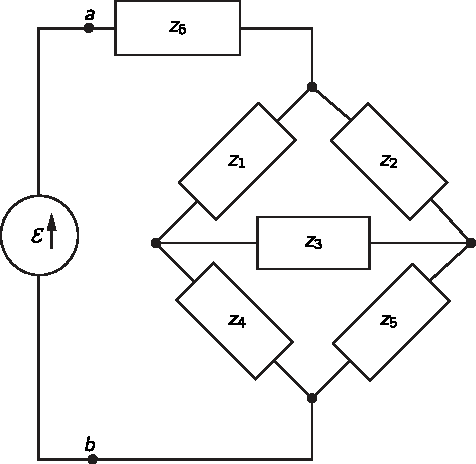
\includegraphics[width=0.7\linewidth]{fyz_fig363.pdf}
    \caption{Můstkové zapojení
             (\cite[s.~403]{Feynman02})}
    \label{fyz:fig363}
  \end{figure}
  
  Takové zapojení se nazývá „\emph{můstek}“. Vyskytuje se v mnoha přístrojích používaných k měření 
  impedancí. V případě můstkového zapojení obvykle klademe otázku: V jakém poměru musí být různé 
  impedance, aby proud impedancí \(Z\) byl nulový? Ponecháme na vás zjistit podmínky, za kterých to 
  nastane.

\newpage
\section{Ekvivalentní obvody}\label{fyz:IIchapXXIIsecIV}
  Představte si, že generátor \(\mathscr{E}\) připojíme k síti obsahující nějaké komplikované 
  spojení impedancí, jako je to schématicky naznačeno na obr. \ref{fyz:fig364a}.
  
  \begin{figure}[hb!] %\ref{fyz:fig364}
    \centering
    \begin{tabular}{cc}
     \subfloat[ ]{\label{fyz:fig364a}
       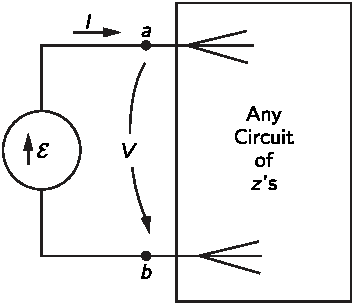
\includegraphics[width=0.4\linewidth]{fyz_fig364a.pdf}}
     \subfloat[ ]{\label{fyz:fig364b}
       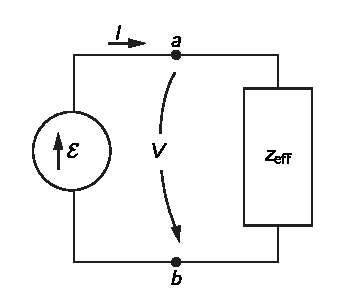
\includegraphics[width=0.4\linewidth]{fyz_fig364b.pdf}}
    \end{tabular}
    \caption{Každá síť složená pouze z pasivních prvků a obsahující dva vývody je ekvivalentní 
             nějaké efektivní impedanci
             (\cite[s.~404]{Feynman02}).}
    \label{fyz:fig364}
  \end{figure}
  
  Všechny rovnice, které dostaneme z Kirchhoffových pravidel, jsou lineární, takže vyřešíme-li je 
  vzhledem k proudu \(I\) procházejícímu generátorem, dostaneme, že \(I\) je přímo úměrné 
  \(\mathscr{E}\). Můžeme tedy psát, že
  \begin{equation*}
    I = \frac{\mathscr{E}}{Z_{ef}},
  \end{equation*}
  kde \(Z_{ef}\) je nyní nějaké komplexní číslo, dané algebraickou funkcí všech prvků v obvodu. 
  (Neobsahuje-li schéma žádné jiné generátory, pouze ten, který je na obrázku vyznačen, nevystupuje 
  zde žádný dodatkový, na \(\mathscr{E}\) nezávisející člen.) Ale tato rovnice je přesně taková, 
  jakou bychom napsali pro obvod na obr. \ref{fyz:fig364b}. Pokud se zajímáme pouze o to, co se 
  děje nalevo od obou svorek \(a\) a \(b\), jsou obě schémata na obr. \ref{fyz:fig364b} 
  ekvivalentní. Můžeme proto formulovat obecný výrok, že každou síť pasivních prvků připojenou ke 
  dvěma svorkám lze nahradit jedinou impedancí \(Z_{ef}\), aniž by se nějak změnily proudy a napětí 
  ve zbytku zapojení. Je pravda, že tento výrok představuje pouhou formulaci toho, co vychází z 
  Kirchhoffových pravidel a konec konců z linearity Maxwellových rovnic. Tuto myšlenku lze zobecnit 
  i na síť, která obsahuje nejen impedance ale i generátory. Představme si, že se na takovou síť 
  díváme „z hlediska“ jedné z impedancí, kterou budeme označovat \(Z_n\) (obr. \ref{fyz:fig365a}). 
  Kdybychom měli řešit rovnice pro celou síť, zjistili bychom, že napětí \(U_n\), mezi dvěma 
  svorkami \(a\) a \(b\) je lineární funkcí proudu \(I\). Můžeme to zapsat takto:
  \begin{equation}\label{fyz:eq489}
    U_n = A - BI_n,
  \end{equation}
  kde \(A\) a \(B\) závisí na generátorech a impedancích, které jsou zapojeny nalevo od svorek. 
  Například pro síť na obr. \ref{fyz:fig361} zjistíme, že \(U_1 = I_1Z_1\). To lze úpravou rovnice 
  (\ref{fyz:eq491}) rozepsat takto: 
  \begin{equation}\label{fyz:eq490}
    U_1 = \left(\frac{Z_2}{Z_2 + Z_3}\mathscr{E_2} - \mathscr{E_1}\right) 
         -\frac{Z_2Z_3}{Z_2 + Z_3}I_1.
  \end{equation}
  
  Úplné řešení pak lze dostat kombinováním tohoto vztahu se vztahem pro impedanci \(Z_1\), totiž 
  \(U_1 = I_1Z_1\), nebo v obecném případě kombinováním vztahu (\ref{fyz:eq489}) se vztahem
  \begin{equation*}
    U_n = I_nZ_n.
  \end{equation*}
  
  \begin{figure}[hb!] %\ref{fyz:fig365}
    \centering
    \begin{tabular}{cc}
     \subfloat[ ]{\label{fyz:fig365a}
       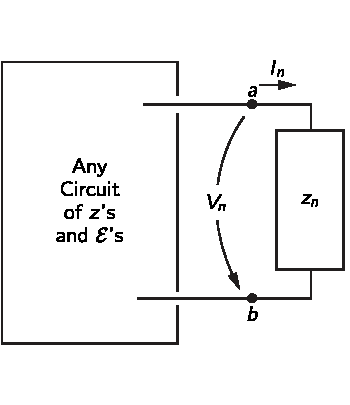
\includegraphics[width=0.4\linewidth]{fyz_fig365a.pdf}}
     \subfloat[ ]{\label{fyz:fig365b}
       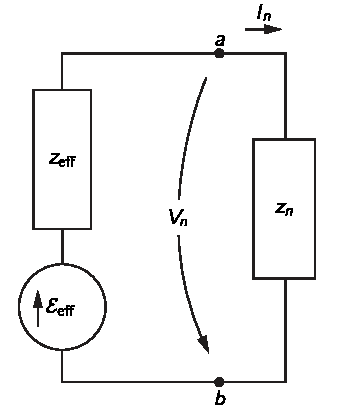
\includegraphics[width=0.4\linewidth]{fyz_fig365b.pdf}}
    \end{tabular}
    \caption{Každou síť se dvěma vývody, obsahující impedance i generátory, lze nahradit 
             generátorem zapojeným do série s impedancí
             (\cite[s.~405]{Feynman02}).}
    \label{fyz:fig365}
  \end{figure}

  Uvažujeme-li případ, že \(Z_n\) se vztahuje na jednoduchý sériový obvod, skládající se z 
  generátoru a impedance, jako na obr. \ref{fyz:fig365b}, vztahu (\ref{fyz:eq489}) bude odpovídat 
  rovnice 
  \begin{equation*}
    U_n = \mathscr{E}_{ef} - I_nZ_{ef}.
  \end{equation*}
  která se s (\ref{fyz:eq489}) shoduje, položíme-li \(\mathscr{E}_{ef} = A\) a \(Z_{ef}= B\). Tedy, 
  zajímáme-li se pouze o to, co se děje napravo od svorek \(a\) a \(b\), je vždy možné nahradit 
  libovolné zapojení z obr. \ref{fyz:fig365} ekvivalentní kombinací generátoru zapojeného v sérii s 
  impedancí.
  
\section{Energie}\label{fyz:IIchapXXIIsecV}
  Viděli jsme, že k tomu, aby v cívce vznikl proud \(I\), musí její vnější obvod dodat energii \(W= 
  \frac{1}{2}LI^2\). Když proud poklesne opět na nulu, uvolní se tato energie zpět do vnějšího 
  obvodu. V ideální indukčnosti nedochází k procesům ztráty energie. Když takovou indukčností 
  prochází střídavý proud, přelévá se energie sem a tam mezi ní a zbytkem obvodu, ale střední 
  rychlost, kterou se do obvodu energie dodává, je rovna nule. Říkáme, že indukčnost je 
  \emph{nedisipativním prvkem} - žádná elektrická energie v ní nedisipuje, tj. neztrácí se. Podobně 
  se do vnějšího obvodu vrací i energie kondenzátoru \(W= \frac{1}{2}CU^2\) při jeho vybíjení. 
  Nachází-li se kondenzátor v obvodu se střídavým proudem, energie do něj vtéká a vytéká, ale 
  sumární tok energie v každém cyklu je rovem nule. Ideální kondenzátor je také 
  \emph{nedisipativním prvkem}. o Víme, že elektromotorické napětí je zdrojem energie. Když proud 
  protéká ve směru elektromotorického napětí, je energie dodávána do vnějšího obvodu rychlostí 
  \(dW/dt =\mathscr{E}I\). Je-li proud poháněn - jinými generátory v obvodu - proti 
  elektromotorickému napětí, bude toto napětí absorbovat energii rychlostí \(\mathscr{E}I\); 
  protože \(I\) je záporné, bude záporné i \(dW/dt\).

  Je-li generátor připojen k rezistoru, jehož odpor je \(R\), prochází jím proud 
  \(I=\mathscr{E}/R\). Energie, již generátor dodává zajednotku času \(\mathscr{E}I\), je 
  rezistorem pohlcována. Tato energie se v něm mění na teplo a z elektrické energie obvodu se 
  ztrácí. Říkáme, že rezistorem se elektrická energie disipuje. Rychlost, kterou se energie mění 
  odporem na teplo, je \(dW/dt = RI^2\).
  
  V obvodu se střídavým proudem je střední rychlost, kterou se energie v odporu ztrácí, rovna 
  střední hodnotě veličiny \(RI^2\) za jeden cyklus. Protože \(I= \hat{I}e^{i\omega t}\) - čímž 
  vlastně myslíme to, že se \(I\) mění jako \(\cos\omega t\) - střední hodnota \(I^2\) za jeden 
  cyklus je rovna \(\abs{\hat{I}}^2/2\), neboť maximální proud je \(\abs{\hat{I}}\) a střední 
  hodnota funkce \(\cos^2\omega t\) je \(1/2\).
  
  Jak je to se ztrátou energie, je-li generátor připojen k libovolné impedanci \(Z\)? („Ztrátou“ 
  rozumíme přeměnu elektrické energie na tepelnou energii.) Každou impedanci \(Z\) lze vyjádřit 
  jako součet její reálné a imaginární části:
  \begin{equation}\label{fyz:eq492}
    Z = R + iX,
  \end{equation}
  kde \(R\) a \(X\) jsou reálná čísla. Z hlediska ekvivalentních obvodů můžeme říci, že každá 
  impedance je ekvivalentní odporu zapojenému do série s ryze imaginární impedancí, kterou nazýváme 
  \textbf{reaktance} (obr. \ref{fyz:fig366}).
  
  \begin{figure}[ht!] %\ref{fyz:fig366}
    \centering
    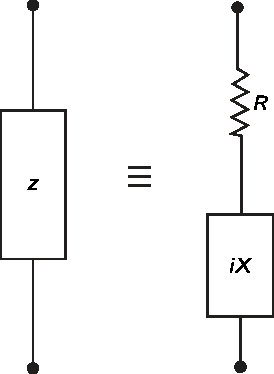
\includegraphics[width=0.3\linewidth]{fyz_fig366.pdf}
    \caption{Každá impedance je ekvivalentní sériovému zapojení čistého odporu a čisté reaktance
             (\cite[s.~406]{Feynman02})}
    \label{fyz:fig366}
  \end{figure}
  
  Už dříve jsme viděli, že impedance každého obvodu obsahujícího pouze indukčnosti \(L\) a kapacity 
  \(C\) je ryze imaginárním číslem. Protože v těchto „\emph{L}“ a „\emph{C}“ nedochází v průměru k 
  žádným ztrátám energie, v čisté reaktanci, skládající se pouze ze samých „\emph{L}“ a „\emph{C}“, 
  žádné ztráty energie nebudou. Můžeme se přesvědčit, že to musí platit pro reaktanci obecně.
  
  Připojí-li se generátor s elektromotorickým napětím \(\mathscr{E}\) k impedanci \(Z\) z obr. 
  \ref{fyz:fig366}, musí elektromotorické napětí souviset s proudem \(I\) z generátoru podle vztahu
  \begin{equation}\label{fyz:eq493}
    \mathscr{E} = I(R + iX). 
  \end{equation}
  Abychom našli střední rychlost, kterou se energie z generátoru odčerpává, potřebujeme znát 
  střední hodnotu součinu \(\mathscr{E}I\). Nyní si musíme dát pozor. Jde-li o takovéto 
  \emph{součiny}, musíme zacházet s reálnými veličinami \(\mathscr{E}(t)\) a \(I(t)\). (Reálné 
  části komplexních funkcí budou představovat skutečné fyzikální veličiny pouze když máme lineární 
  rovnice; nyní však máme součiny, které zajisté nejsou lineární.)
  
  Předpokládejme, že jsme si vybrali počátek počítání času \(t\) tak, aby amplituda \(\hat{I}\) 
  byla reálným číslem, řekněme \(I_0\); pak skutečný průběh \(I\) v čase udává vztah
  \begin{equation}\label{fyz:eq494}
  I = I_0\cos\omega t.
  \end{equation}
  Elektromotorické napětí v (\ref{fyz:eq492}) je rovno reálné části výrazu
  \begin{equation*}
    I_0e^{i\omega t}(R + iX)
  \end{equation*}
  tj.
  \begin{equation}\label{fyz:eq495}
    \mathscr{E} = I_0R\cos\omega t - I_0X\sin\omega t.
  \end{equation}
  
  Dva členy ve vztahu (\ref{fyz:eq495}) představují úbytky napětí na \(R\) a \(X\) z obr. 
  \ref{fyz:fig366}. Vidíme, že úbytek napětí na odporu je ve fázi s proudem, zatímco úbytek napětí 
  na reaktivní části je vzhledem k proudu posunut. Střední ztráta energie generátoru zajednotku 
  času \(\left\langle P\right\rangle_{\text{stř}}\) je rovna integrálu součinu \(\mathscr{E}I\) 
  počítanému za jeden cyklus a vydělenému periodou \(T\), tj.
  
  \begin{align*}
    \left\langle P\right\rangle_{\text{stř}} 
      &= \frac{1}{T}\int_0^T\mathscr{E}I\dd{t}             \\
      &= \frac{1}{T}\int_0^TI_0^2R\cos^2\omega t\dd{t}     
       - \frac{1}{T}\int_0^TI_0^2X\cos\omega t\sin\omega t\dd{t}
  \end{align*}
  
  První integrál je roven \(I_0^2R/2\) a druhý integrál je roven. Proto střední ztráta energie 
  v impedanci \(Z= R+iX\) závisí pouze na reálné části \(Z\) a je rovna \(I_0^2R/2\), což souhlasí 
  s naším dřívějším výsledkem pro ztrátu energie v odporu. V reaktivní části nedochází k žádné 
  ztrátě energie.
  
\section{Řetězový obvod}\label{fyz:IIchapXXIIsecVI}
  Nyní bychom rádi prozkoumali zajímavé schéma, které lze analyzovat pomocí sériových a paralelních 
  zapojení. Začněme, řekněme s obvodem, jehož schéma je na obr. \ref{fyz:fig367a}. Ihned je vidět, 
  že impedance od svorky \(a\) po svorku \(b\) je prostě rovna \(Z_1 + Z_2\). Nyní vezměme trochu 
  složitější obvod, tj. ten jehož schéma je na obr. \ref{fyz:fig367b}. Mohli bychom jej analyzovat 
  pomocí Kirchhoffových pravidel, ale je také dostatečně snadný na to, aby se dal zvládnout 
  uvažováním o sériových a paralelních zapojeních. Obě impedance na pravém konci lze nahradit 
  jedinou impedancí \(Z_3 = Z_1 + Z_2\), jako je tomu na pravé části obr. \ref{fyz:fig367b}. Nato 
  můžeme obě impedance \(Z_2\) a \(Z_3\) nahradit jejich ekvivalentní „paralelní“ impedancí 
  \(Z_4\), což ukazuje levá část obrázku \ref{fyz:fig367c}. Konečně \(Z_1\) a \(Z_4\) jsou 
  ekvivalentní jediné impedanci \(Z_5\), což je vidět na pravé části obrázku \ref{fyz:fig367c}.

  \begin{figure}[ht!] %\ref{fyz:fig368}
    \centering
    \begin{tabular}{c}
     \subfloat[ ]{\label{fyz:fig367a}
       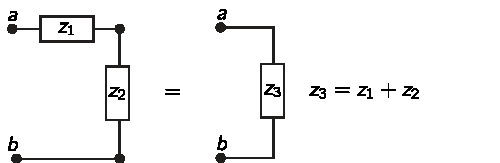
\includegraphics[width=0.6\linewidth]{fyz_fig367a.pdf}}   \\
     \subfloat[ ]{\label{fyz:fig367b}
       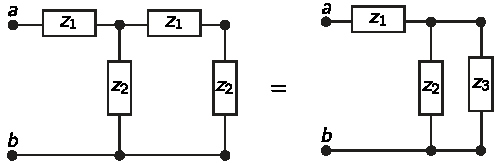
\includegraphics[width=0.6\linewidth]{fyz_fig367b.pdf}}   \\
     \subfloat[ ]{\label{fyz:fig367c}
       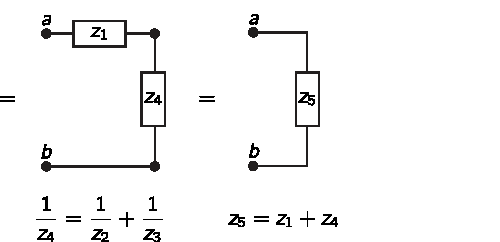
\includegraphics[width=0.6\linewidth]{fyz_fig367c.pdf}}
    \end{tabular}
    \caption{Efektivní impedance řetězového obvodu
             (\cite[s.~407]{Feynman02})}
    \label{fyz:fig367}
  \end{figure}
  
  Nyní můžeme položit zábavnou otázku: Co by se stalo, kdybychom do sítě na levé části obr. 
  \ref{fyz:fig367b} neustále přidávali další sekce, jako jsme to čárkovaně vyznačili na 
  obr.\ref{fyz:fig368a}? Lze takovou nekonečnou síť řešit? Tak těžké to není. Především si 
  všimněme, že se taková nekonečná síť nezmění, přidáme-li na její „přední“ konec ještě jednu 
  sekci. Opravdu, když přidáme ještě jednu sekci k nekonečné síti, je to stále ještě tatáž 
  nekonečná síť.
  
  \begin{figure}[ht!] %\ref{fyz:fig368}
    \centering
    \begin{tabular}{c}
     \subfloat[ ]{\label{fyz:fig368a}
       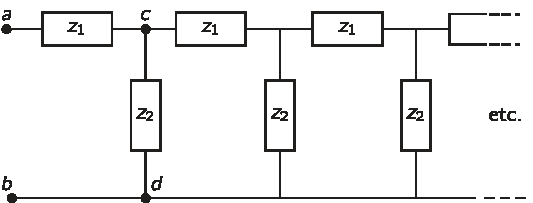
\includegraphics[width=0.6\linewidth]{fyz_fig368a.pdf}}   \\
     \subfloat[ ]{\label{fyz:fig368b}
       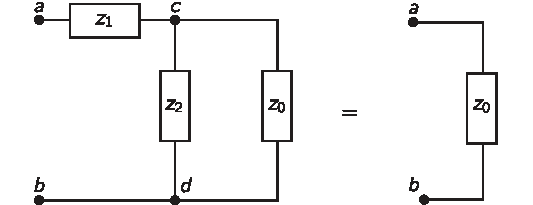
\includegraphics[width=0.6\linewidth]{fyz_fig368b.pdf}}
    \end{tabular}
    \caption{Efektivní impedance nekonečného řetězového obvodu
             (\cite[s.~408]{Feynman02}).}
    \label{fyz:fig368}
  \end{figure}

  Impedanci nekonečné sítě mezi svorkami \(a\) a \(b\) označme \(Z_0\); pak ale impedance všeho, co 
  se nachází vpravo od svorek \(c\) a \(d\) je také \(Z_0\). Proto pokud jde o přední konec, můžeme 
  naši síť chápat tak, jak ukazuje obr. \ref{fyz:fig368b}. Přidáme-li výsledek paralelního zapojení 
  \(Z_2\) a \(Z_0\) do série s \(Z_1\), můžeme pro impedanci tohoto zapojení ihned napsat:
  \begin{equation*}
    Z = Z_1 + \dfrac{1}{\dfrac{1}{Z_2}+\dfrac{1}{Z_0}} \quad\text{nebo}\quad
    Z = Z_1 + \dfrac{Z_2Z_0}{Z_2 + Z_0}.
  \end{equation*}
  Ale tato impedance je také rovna \(Z_0\) a proto dostáváme rovnici
  \begin{equation*}
    Z_0 = Z_1 + \dfrac{Z_2Z_0}{Z_2 + Z_0}.
  \end{equation*}
  Jejím řešením vzhledem k \(Z_0\) vychází, že
  \begin{equation}\label{fyz:eq498}
    Z_0 = \dfrac{Z_1}{2} + \sqrt{(Z_1^2/4) + Z_1Z_2}.
  \end{equation}
  
  Tak jsme našli výraz pro impedanci nekonečného řetězového obvodu skládajícího se z opakujících se 
  sériových a paralelních impedancí. Impedance \(Z_0\) se nazývá \emph{charakteristická impedance} 
  takové nekonečné sítě. 
  
  \begin{figure}[ht!] %\ref{fyz:fig369}
    \centering
    \begin{tabular}{c}
     \subfloat[ ]{\label{fyz:fig369a}
       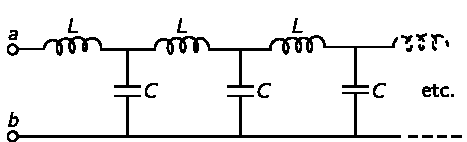
\includegraphics[width=0.7\linewidth]{fyz_fig369a.pdf}}  \\
     \subfloat[ ]{\label{fyz:fig369b}
       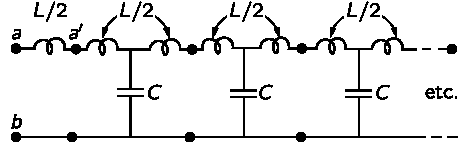
\includegraphics[width=0.7\linewidth]{fyz_fig369b.pdf}}
    \end{tabular}
    \caption{Řetězový obvod \(LC\) nakreslený dvěma ekvivalentními způsoby
             (\cite[s.~409]{Feynman02}).}
    \label{fyz:fig369}
  \end{figure}
  Prozkoumejme specifický případ, kdy je sériovým prvkem indukčnost \(L\) a paralelním je kapacita 
  \(C\) (obr. \ref{fyz:fig369a}). Impedanci nekonečné sítě v tomto případě najdeme, když dosadíme 
  \(Z_1 =i\omega L\) a \(Z_2 = 1/i\omega C\). Všimněme si, že první člen na pravé straně vztahu 
  (\ref{fyz:eq498}), tj. \(Z_1/2\) je roven právě polovině impedance prvního prvku. Proto by bylo 
  přirozenější nebo alespoň jednodušší, kdybychom nekonečnou síť kreslili tak, jako na obr. 
  \ref{fyz:fig369b}.
  
  Při pohledu na tuto nekonečnou síť ze svorky \(a'\) bychom pozorovali tuto charakteristickou 
  impedanci
  \begin{equation}\label{fyz:eq499}
    Z_0 = \sqrt{L/C) - (\omega^2L^2/4)}.
  \end{equation}
  V závislosti na frekvenci \(\omega\) existují dva zajímavé případy. Je-li \(\omega^2\) menší než 
  \(4/LC\), bude druhý člen pod odmocninou menší než první a impedance \(Z_0\) bude reálná. Naproti 
  tomu, když \(\omega^2\) je větší než \(4/LC\), impedance \(Z_0\) bude ryze imaginární a lze ji 
  vyjádřit jako:
  \begin{equation*}
    Z_0 = i\sqrt{(\omega^2L^2/4) – (L/C)}.
  \end{equation*}
  
  Už jsme řekli, že síť obsahující jen imaginární impedance, tj. induktance a kapacitance, bude mít 
  ryze imaginární impedanci. Jak tedy může síť, kterou nyní zkoumáme - a která má pouze samá \(L\) 
  a \(C\) - mít impedanci při frekvencích nižších než \(4/LC\) rovnu čisté rezistanci? Při vyšších 
  frekvencích je impedance ryze imaginární, což plně souhlasí s naším dřívějším tvrzením. Při 
  nižších frekvencích je však impedance rovna čisté rezistanci a bude proto absorbovat energii. Ale 
  jak tato síť může nepřetržitě absorbovat energii - tak,jak je tomu v případě odporu - když je 
  sestavena pouze z indukčností a kapacit? Je to proto, že jde o nekonečný počet indukčností a 
  kapacit, takže je-li k takové síti připojen zdroj, dodává nejdříve energii do první indukčnosti a 
  kapacity, pak do druhé, do třetí atd. V takové síti se energie z generátoru absorbuje spojitě a 
  konstantní rychlostí. Stále protéká do sítě a ukládá se v indukčnostech a kapacitách podél vedení.
  
  Tato představa naznačuje zajímavou věc o procesech v takové síti. Když k přednímu konci sítě 
  připojíme zdroj, je třeba očekávat, že jeho účinky se budou sítí šířit k jejímu nekonečnému 
  konci. Postup tohoto vlnění po vedení se v mnohém podobá vyzařování antény, která absorbuje 
  energii ze svého napájecího zdroje; vznik takového vlnění totiž očekáváme, když je impedance 
  reálná, což nastává, když je \(\omega\) menší než \(\sqrt{4/LC}\). Ale když je impedance ryze 
  imaginární, což nastává při hodnotách \(\omega\) větších než \(\sqrt{4/LC}\), nelze žádné takové 
  šíření očekávat.

\section{Filtry}\label{fyz:IIchapXXIIsecVII}
  V předešlém článku jsme viděli, že nekonečný řetězový obvod na obr. \ref{fyz:fig369} absorbuje 
  energii nepřetržitě, je-li napájen při frekvenci ležící pod určitou kritickou frekvencí 
  \(\sqrt{4/LC}\), kterou budeme nazývat mezní frekvencí \(\omega_0\). Naznačili jsme, že tento 
  efekt lze pochopit pomocí představy o spojitém přenosu energie podél vedení. Na druhé straně, při 
  \(\omega>\omega_0\) k nepřetržitému pohlcování energie nedochází; je třeba čekat, že tehdy asi 
  proudy nebudou „pronikat“ příliš daleko do vedení. Podívejme se, zda jsou tyto představy správné.
  
  \begin{figure}[ht!] %\ref{fyz:fig370}
    \centering
    \begin{tabular}{c}
     \subfloat[ ]{\label{fyz:fig370a}
       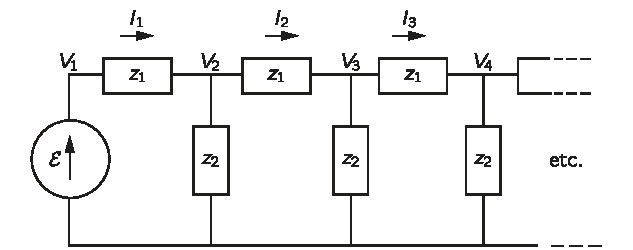
\includegraphics[width=0.7\linewidth]{fyz_fig370a.pdf}} \\
     \subfloat[ ]{\label{fyz:fig370b}
       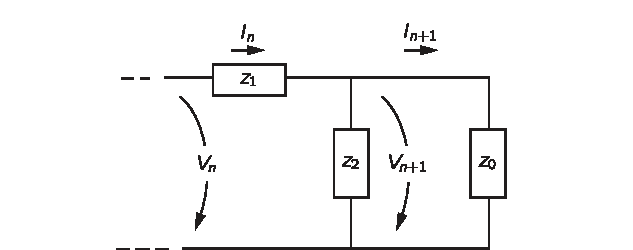
\includegraphics[width=0.7\linewidth]{fyz_fig370b.pdf}}
    \end{tabular}
    \caption{K odvození činitele přenosu řetězového obvodu
             (\cite[s.~410]{Feynman02}).}
    \label{fyz:fig370}
  \end{figure}
  
  Představte si, že jsme přední konec článku připojili k nějakému generátoru střídavého proudu a 
  ptáme se, jak bude vypadat napětí, řekněme na \num{754}-té sekci obvodu. Pokud jde o nekonečnou 
  síť, děje se s napětím při přechodu od jedné sekce k druhé totéž: podívejme se tedy, k čemu 
  dochází, postoupíme-li od nějaké sekce, řekněme \(n\)-té, k následující. Proudy \(I_n\) a napětí 
  \(U_n\), budeme definovat tak, jak je to vyznačeno na obr. \ref{fyz:fig370a}.
  
  Napětí \(U_{n+1}\) můžeme dostat z \(U_n\), vzpomeneme-li si, že vždy lze zbytek řetězového 
  obvodu po \(n\)-té sekci nahradit jeho charakteristickou impedancí \(Z_0\); pak je nutné 
  analyzovat pouze obvod na obr. \ref{fyz:fig370b}. Především vidíme, že každé \(U_n\) je rovno 
  \(I_nZ_0\), neboť jde o napětí na impedanci \(Z_0\). Kromě toho rozdíl mezi \(U_n\), a 
  \(U_{n+1}\) je roven právě \(I_nZ_1\):
  \begin{align*}
    U_n - U_{n+1}       &= I_nZ_1 = U_n\frac{Z_1}{Z_0}.  \\
    \shortintertext{Pro poměr obou napětí dostáváme vyjádření} 
    \frac{U_{n+1}}{U_n} &= 1 - \frac{Z_1}{Z_0} = \frac{Z_0 -Z_1}{Z_0}.
  \end{align*}
  Tento poměr můžeme nazvat \textbf{činitelem přenosu} pro jednu sekci řetězového obvodu a označíme 
  jej \(\alpha\). Přirozeně, je pro všechny sekce stejný: 
  \begin{align*}
    \alpha  &= \frac{Z_0 -Z_1}{Z_0}.  \\
    \shortintertext{Pak je napětí po \(n\)-té sekci} 
    U_n     &= \alpha^n\mathscr{E}.
  \end{align*}
  Nyní můžeme najít napětí po \num{754} sekcích; je rovno součinu \(\mathscr{E}\) a \num{754}-té 
  mocniny \(\alpha\). 
  
  Jaké bude \(\alpha\) pro L-C síť z obr. \ref{fyz:fig369a}? Dosadíme-li \(Z_0\) ze vztahu 
  (\ref{fyz:eq498}) a \(Z_1 =i\omega L\), dostaneme
  \begin{equation}\label{fyz:eq500}
    \alpha = \dfrac{\sqrt{L/C) - (\omega^2L^2/4)} - i(\omega L/2)}
                   {\sqrt{L/C) - (\omega^2L^2/4)} + i(\omega L/2)}
  \end{equation}
  Když napájecí frekvence leží pod hraniční frekvencí \(\omega_0 =\sqrt{4/LC}\), je odmocnina 
  reálným číslem a komplexní čísla v činiteli a ve jmenovateli mají stejné velikosti. Proto je 
  absolutní hodnota a rovna 1 a můžeme psát, že
  \begin{equation*}
    \alpha = e^{i\delta}
  \end{equation*}
  což znamená, že velikost napětí je pro každou sekci tatáž a mění se pouze jeho fáze. Změna fáze 
  \(\delta\) je vlastně záporné číslo a představuje opožďování napětí při jeho postupu v síti. 
  
  Pro frekvence ležící nad hraniční frekvencí a je lepší zkrátit jmenovatele i čitatele ve vztahu 
  (\ref{fyz:eq500}) imaginární jednotkou \(i\) a (\ref{fyz:eq500}) přepsat do tvaru
  \begin{equation}\label{fyz:eq501}
    \alpha = \dfrac{\sqrt{(\omega^2L^2/4) – (L/C)} - (\omega L/2)}
                   {\sqrt{(\omega^2L^2/4) – (L/C)} + (\omega L/2)}
  \end{equation}
  Činitel přenosu \(\alpha\) je nyní reálný a je menší než jedna. To znamená, že napětí na každé 
  sekci je ve srovnání s napětím na předcházející sekci menší v poměru \(\alpha\). Pro každou 
  frekvenci větší než \(\omega_0\) napětí při postupu sítí rychle zaniká. Graf absolutní hodnoty 
  \(\alpha\) jako funkce frekvence vypadá tak, jak je znázorněno na obr. \ref{fyz:fig371}. 
  
  \begin{figure}[ht!] %\ref{fyz:fig371}
    \centering
    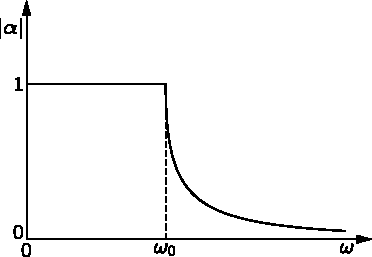
\includegraphics[width=0.5\linewidth]{fyz_fig371.pdf}
    \caption{Činitel přenosu jedné sekce řetězového obvodu LC
             (\cite[s.~411]{Feynman02})}
    \label{fyz:fig371}
  \end{figure}
  
  Vidíme, že chování \(\alpha\) jak nad tak i pod \(\omega_0\) souhlasí s naší interpretací, že síť 
  energii přenáší při \(\omega<\omega_0\) a přehrazuje při \(\omega>\omega_0\). Říkáme, že taková 
  síť nízké frekvence propouští a vysoké frekvence odfiltrovává.
  
  Každá síť, která je vyprojektována tak, aby se její charakteristiky předepsaným způsobem měnily s 
  frekvencí, se nazývá \textbf{filtr}. My jsme analyzovali filtr nízkých frekvencí, tzv. 
  \emph{dolní propust}.
  
  Možná nás udivuje, proč provádíme celou tuto diskuzi nekonečné sítě, kterou nelze prakticky 
  realizovat. Je to v tom, že tytéž charakteristiky nacházíme i u konečné sítě, je-li zakončena 
  impedancí rovnající se charakteristické impedanci \(Z_0\). V praxi se však nepodaří přesně 
  reprodukovat charakteristickou impedanci pomocí několika jednoduchých prvků, jako jsou \(R\), 
  \(L\) a \(C\). Ale často toho lze s velmi dobrým přiblížením dosáhnout pro určitý rozsah 
  frekvencí. Tak lze sestrojit konečnou filtrační síť, jejíž vlastnosti jsou téměř stejné,jako má 
  nekonečná síť. Například řetězový obvod LC se v mnohém chová tak, jak jsme to popsali, je-li 
  zakončen čistou rezistancí \(R = \sqrt{L/C}\).
    
  \begin{figure}[ht!] %\ref{fyz:fig372}
    \centering
    \begin{tabular}{c}
     \subfloat[ ]{\label{fyz:fig372a}
       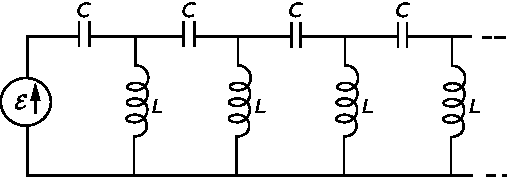
\includegraphics[width=0.7\linewidth]{fyz_fig372a.pdf}} \\
     \subfloat[ ]{\label{fyz:fig372b}
       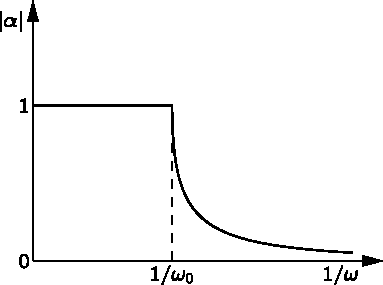
\includegraphics[width=0.5\linewidth]{fyz_fig372b.pdf}}
    \end{tabular}
    \caption{a) horní propust, b) její součinitel přenosu jako funkce \(1/\omega\)
             (\cite[s.~411]{Feynman02}).}
    \label{fyz:fig372}
  \end{figure}
  
  Když v našem obvodu LC navzájem vyměníme polohy \(L\) a \(C\), aby vznikl obvod ukázaný na obr. 
  \ref{fyz:fig372a}, můžeme dostat filtr, který přenáší \emph{vysoké} frekvence a přehrazuje 
  \emph{nízké} frekvence. Už pomocí našich dosavadních výsledků lze snadno zjistit, co se v této 
  síti děje. Patrně jsme už zjistili, že kdykoliv \(L\) nahrazujeme \(C\) a naopak, měníme každé 
  \(i\omega\) na \(1/i\omega\), resp. naopak. Konkrétně, změníme-li na obr. \ref{fyz:fig371} 
  označení horizontální osy na \(1/\omega\) (obr. \ref{fyz:fig372b}), můžeme nahlédnout, jak se 
  bude měnit \(\alpha\) s frekvencí. 
  
  Dolní a horní propust, které jsou tu popsány, nacházejí rozmanité technické využití. Dolní 
  propust LC se často používá jako „vyhlazovací“ filtr v napájecích zdrojích stejnosměrného proudu. 
  Potřebujeme-li vyrábět stejnosměrný proud ze zdroje střídavého proudu, připojíme na začátek 
  usměrňovač, který proudu dovoluje téci jen jedním směrem. Z usměrňovače dostaneme posloupnost 
  impulzů, které vypadají jako funkce \(U(t)\) znázorněná na obr. \ref{fyz:fig373} a představují 
  nedokonalý stejnosměrný proud, neboť kmitá nahoru a dolů. Dejme tomu, že bychom rádi dostali 
  krásný, čistý stejnosměrný proud, jaký poskytuje akumulátorová baterie. Můžeme se k tomu 
  přiblížit, vložíme-li mezi usměrňovač a zátěž dolní propust. 
  
  Z kapitoly \ref{fyz:IchapL} dílu \ref{part:FYZI} víme, že takovou funkci času, jako je na obr. 
  \ref{fyz:fig373}, lze vyjádřit jako následující superpozice: stálé napětí plus sinusová vlna plus 
  sinusová vlna o vyšším kmitočtu plus sinusová vlna o ještě vyšším kmitočtu atd., tj. jako 
  \textbf{Fourierova řada}. Je-li náš filtr lineární (když jak jsme předpokládali - se hodnoty 
  \(L\) a \(C\) nemění při změnách proudů a napětí), pak to, co z filtru vychází, představuje 
  superpozici výstupů od každé složky na jeho vstupu.
  
  \begin{figure}[ht!] %\ref{fyz:fig373}
    \centering
    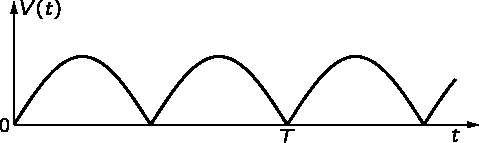
\includegraphics[width=0.7\linewidth]{fyz_fig373.pdf}
    \caption{Výstupní napětí dvoucestného usměrňovače
             (\cite[s.~412]{Feynman02})}
    \label{fyz:fig373}
  \end{figure}
  
  Zabezpečíme-li, aby mezní frekvence \(\omega_0\) pro náš filtr ležela hodně pod nejnižší 
  frekvencí ve funkci \(U(t)\) bude stejnosměrný proud (pro nějž \(\omega = 0\)) filtrem procházet 
  pěkně, ale amplituda první harmonické bude značně seříznuta. A amplitudy vyšších harmonických 
  budou seříznuty ještě víc. Výstup tedy můžeme dostat libovolně hladký; závisí to jen na tom, 
  kolik filtračních členů jsme ochotni koupit.
  
  Horní propust se používá, je-li třeba přehradit některé nízké frekvence. Lze jej například použít 
  v gramofonovém zesilovači, aby se propouštěla hudba a současně se zadržoval nízkofrekvenční hukot 
  vznikající chvěním motorku otáčejícího kotoučem.
  
  \begin{figure}[ht!] %\ref{fyz:fig374}
    \centering
    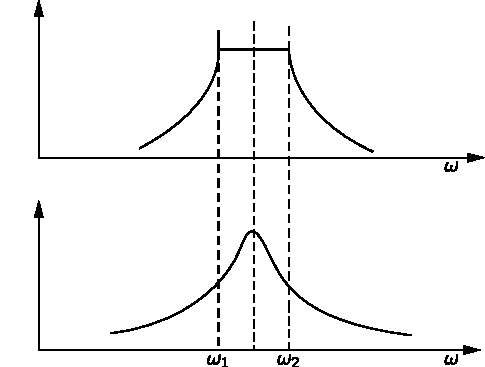
\includegraphics[width=0.7\linewidth]{fyz_fig374.pdf}
    \caption{nahoře) pásmová propust, dole) prostá rezonanční propust
             (\cite[s.~412]{Feynman02}).}
    \label{fyz:fig374}
  \end{figure}
  
  Lze vyrobit i pásmové propusti, které přehrazují frekvence ležící pod nějakou frekvencí 
  \(\omega_1\) a nad jinou frekvencí \(\omega_2\). (vyšší než \(\omega_1\)), ale mezi \(\omega_1\) 
  a \(\omega_2\) propouštějí. Toho lze docílit snadno složením horní a dolní propusti dohromady. 
  Ale častěji se to provádí pomocí řetězového obvodu, v němž jsou komplikovanější impedance \(Z_1\) 
  a \(Z_2\) - každá představuje kombinaci několika \(L\) a \(C\). Činitel přenosu takové pásmové 
  propusti bude vypadat tak jako graf na horní části obr. \ref{fyz:fig374}. Lze ji použít k 
  oddělení signálů, které zabírají pouze určitý frekvenční interval, například z mnoha kanálů ve 
  vysokofrekvenčním telefonním kabelu nebo modulované nosné vlny rozhlasového vysílání. 
  
  V kapitole \ref{fyz:IchapXXV} dílu \ref{part:FYZI} jsme viděli, že takového filtrování lze 
  docílit i využitím selektivnosti obyčejné rezonanční křivky, kterou jsme pro porovnání nakreslili 
  na dolní části obr. \ref{fyz:fig374}. Pro některé účely však rezonanční filtr není tak dobrý jako 
  pásmový. Jistě si vzpomínáme (kapitola \ref{fyz:IchapXLVIII}, díl \ref{part:FYZI}), že je-li 
  nosná vlna o frekvenci \(\omega_n\), modulována „signálovou“ frekvencí \(\omega_m\), výsledný 
  signál neobsahuje jen nosnou frekvenci, ale i frekvence dvou bočních \(\omega_n+\omega_m\) a 
  \(\omega_n-\omega_m\). V rezonančním filtru se tato boční pásma vždy trochu zeslabují a zeslabení 
  je tím větší, čím vyšší je frekvence signálu, o čemž se můžete přesvědčit na obrázku. Takový 
  filtr tedy nemá dobrou frekvenční charakteristiku. Vyšší hudební tóny se přes něj nedostanou. Ale 
  provádí-li se filtrování pomocí pásmového filtru zkonstruovaného tak, aby šířka 
  \(\omega_2-\omega_1\) byla alespoň dvojnásobkem signálové frekvence, bude frekvenční 
  charakteristika pro příslušné signály „plochá“. 
  
  Je nutné udělat ještě jednu poznámku o řetězovém obvodu: LC obvod z obr. \ref{fyz:fig369} 
  přibližně představuje i \textbf{přenosové vedení}. Máme-li dlouhý vodič uložený rovnoběžně s 
  jiným vodičem, například drát v koaxiálním kabelu nebo drát zavěšený nad zemí, bude mezi těmito 
  vodiči existovat určitá kapacita i určitá indukčnost způsobená magnetickým polem mezi nimi. 
  Představíme-li si toto vedení rozdělené na malé části délky \(\Delta l\), bude každá délka 
  vypadat jako sekce LC obvodu se sériovou indukčností \(\Delta L\) a paralelní kapacitou \(\Delta 
  C\). Pak lze použít naše výsledky pro řetězový filtr. Vezmeme-li limitu, když se \(\Delta l\) 
  blíží k nule, dostaneme dobrý popis přenosového vedení. Všimněte si, že když se \(\Delta l\) víc 
  a víc zkracuje, zmenšují se zároveň i hodnoty \(\Delta L\) a \(\Delta C\), ale vždy ve stejném 
  poměru, takže podíl \(\Delta L/\Delta C\) se pak nemění. Proto vezmeme-li limitu rovnice 
  (\ref{fyz:eq499}), když se \(\Delta L\) a \(\Delta C\) blíží k nule, zjistíme, že 
  charakteristická impedance \(Z_0\) je rovna čisté rezistanci, jejíž velikost je \(\sqrt{\Delta 
  L/\Delta C}\). Poměr \(\Delta L/\Delta C\) můžeme vyjádřit jako \(L_0/C_0\) kde \(L_0\) a \(C_0\) 
  označují indukčnost a kapacitu jednotkové délky vedení. Pak dostaneme vztah
  
  \begin{equation}\label{fyz:eq502}
    Z_0 = \sqrt{\dfrac{L_0}{C_0}}.
  \end{equation}
  
  Také si všimněme, že když se \(\Delta L\) a \(\Delta C\) blíží nule, jde mezní frekvence 
  \(\omega_0 = \sqrt{4/LC}\) k nekonečnu. Pro ideální přenosové vedení neexistuje žádná mezní 
  frekvence.
  
\newpage
\section{Jiné prvky obvodů}\label{fyz:IIchapXXIIsecVIII}
  Dosud jsme definovali v obvodu jen ideální impedance - indukčnost, kapacitu a odpor, jakož i 
  ideální generátor napětí. Nyní chceme ukázat, že jiné prvky, například vzájemné indukčnosti nebo 
  tranzistory nebo elektronky, také lze popsat pomocí těchto základních prvků. Představme si, že 
  máme dvě cívky a že část indukčního toku z jedné cívky - ať už úmyslně nebo z jiné příčiny - 
  protíná druhou cívku (obr. \ref{fyz:fig375a}). Pak budou mít obě cívky vzájemnou indukčnost 
  \(M\), takže když se v jedné z nich mění proud, ve druhé se bude generovat napětí. Můžeme takový 
  efekt vyjádřit v našich ekvivalentních obvodech? Můžeme, a to následujícím způsobem. Viděli jsme, 
  že elektromotorické napětí indukované v každé z obou vzájemně na sebe působících cívek lze 
  vyjádřit jako součet dvou částí:
  \begin{subequations}\label{fyz:eq496}
    \begin{align}
      \mathscr{E}_1 &=-L_1\der{I_1}{t}\pm M\der{I_2}{t}      \label{fyz:eq497a} \\
      \mathscr{E}_2 &=-L_2\der{I_2}{t}\pm M\der{I_1}{t}.     \label{fyz:eq497b}
    \end{align}
  \end{subequations}

  První člen pochází z vlastní indukčnosti dané cívky a druhý ze vzájemné indukčnosti s druhou 
  cívkou. Znaménko druhého členu může být plus nebo minus v závislosti na tom, jak magnetický tok z 
  jedné cívky protíná druhou cívku. Provedeme-li tytéž aproximace, jaké jsme použili při popisu 
  ideální indukčnosti, můžeme tvrdit, že rozdíl potenciálů svorek každé cívky je roven 
  elektromotorickému napětí v cívce. Pak jsou obě rovnice v soustavě (\ref{fyz:eq496}) stejné, jako 
  bychom dostali pro obvod na obr. \ref{fyz:fig375b} za předpokladu, že elektromotorické napětí v 
  každém z obou nakreslených obvodů závisí na proudu v druhém obvodu podle vztahů
  \begin{equation}\label{fyz:eq497}
    \mathscr{E}_1 = \pm i\omega MI_2, \quad \mathscr{E}_2 = \pm i\omega MI_1.
  \end{equation}
  
  \begin{figure}[ht!] %\ref{fyz:fig375}
    \centering
    \begin{tabular}{cc}
     \subfloat[ ]{\label{fyz:fig375a}
       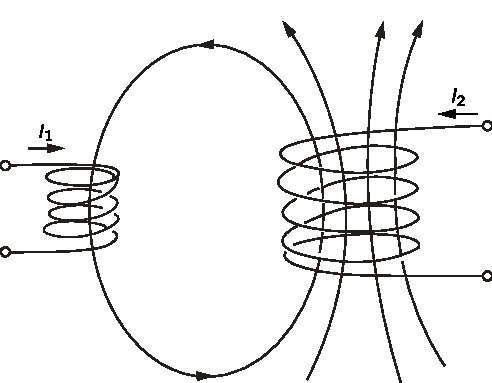
\includegraphics[width=0.45\linewidth]{fyz_fig375a.pdf}}
     \subfloat[ ]{\label{fyz:fig375b}
       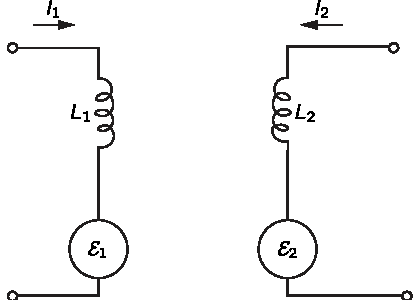
\includegraphics[width=0.45\linewidth]{fyz_fig375b.pdf}}
    \end{tabular}
    \caption{Ekvivalentní obvod vzájemné indukčnosti
             (\cite[s.~412]{Feynman02}).}
    \label{fyz:fig375}
  \end{figure}

  Co můžeme udělat, je toto: Účinek vlastní indukčnosti vyjádřit normálním způsobem a účinek 
  vzájemné indukčnosti nahradit pomocným ideálním generátorem napětí. Kromě toho musíme, 
  samozřejmě, mít i rovnici, která toto elektromotorické napětí uvádí do souvislosti s proudem v 
  nějaké části obvodu; ale pokud je tato rovnice lineární, k našim rovnicím pro obvod jsme pouze 
  přidali další lineární rovnice a všechny z našich dřívějších závěrů o ekvivalentních obvodech 
  apod. zůstávají v platnosti. 

  Kromě vzájemných indukčností mohou existovati vzájemné kapacity. Dosud, když jsme hovořili o 
  kondenzátorech,jsme si vždy představovali, že jde jen o dvě elektrody. Avšak v mnoha situacích, 
  například v elektronce, se může blízko u sebe nacházet mnoho elektrod. Vložíme-li na jakoukoliv 
  elektrický náboj, bude její elektrické pole indukovat náboje na každé další elektrodě a 
  ovlivňovat její potenciál. Jako příklad prozkoumáme takovou sestavu elektrod, jakou znázorňuje 
  obr. \ref{fyz:fig376a}. Představte si, že tyto čtyři elektrody jsou připojeny k vnějším obvodům 
  pomocí vodičů \(A\), \(B\), \(C\) a \(D\). Pokud nás zajímají jen elektrostatické efekty, ukazuje 
  ekvivalentní obvod takové soustavy elektrod na obrázku obr. \ref{fyz:fig376b}. Vzájemné 
  elektrostatické působení každé elektrody na každou další z těchto elektrod je ekvivalentní 
  existenci kapacity mezi těmito elektrodami.
  
  \begin{figure}[ht!] %\ref{fyz:fig376}
    \centering
    \begin{tabular}{cc}
     \subfloat[ ]{\label{fyz:fig376a}
       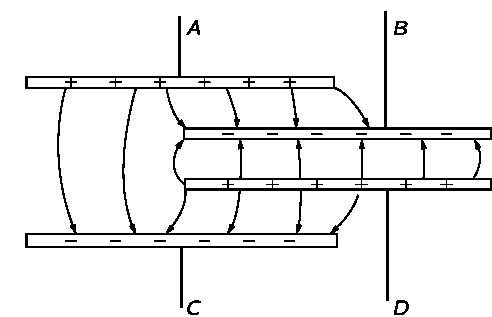
\includegraphics[width=0.6\linewidth]{fyz_fig376a.pdf}}
     \subfloat[ ]{\label{fyz:fig376b}
       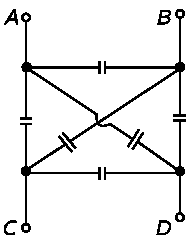
\includegraphics[width=0.3\linewidth]{fyz_fig376b.pdf}}
    \end{tabular}
    \caption{Ekvivalentní obvod vzájemné kapacity
             (\cite[s.~415]{Feynman02}).}
    \label{fyz:fig376}
  \end{figure}

  Konečně prozkoumáme, jak bychom měli v obvodech se střídavými proudy reprezentovat taková složitá 
  zařízení, jako jsou \emph{tranzistory} a \emph{elektronky}. Na začátku je třeba zdůraznit, že 
  tato zařízení často pracují takovým způsobem, že vztah mezi proudy a napětími vůbec není 
  lineární. V takových případech ta z našich tvrzení, která závisí na lineárních rovnicích 
  přestávají platit. Na druhé straně v mnoha aplikacích jsou funkční charakteristiky dostatečně 
  lineární, abychom mohli tranzistory a elektronky pokládat za lineární zařízení. Myslíme tím, že 
  střídavé proudy řekněme v anodovém obvodu elektronky jsou přímo úměrné napětím na jiných 
  elektrodách, například mřížkovému napětí a anodovému napětí. Existují-li takové lineární vztahy, 
  můžeme včlenit příslušné zařízení do naší reprezentace pomocí ekvivalentního obvodu.

  \begin{figure}[ht!] %\ref{fyz:fig377}
    \centering
    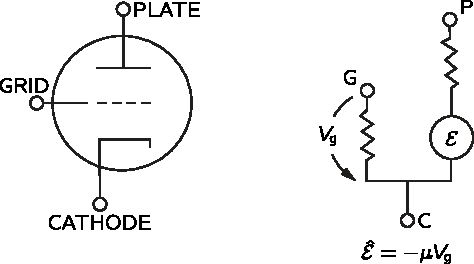
\includegraphics[width=0.6\linewidth]{fyz_fig377.pdf}
    \caption{Ekvivalentní obvod elektronky při nízkých frekvencích
             (\cite[s.~415]{Feynman02})}
    \label{fyz:fig377}
  \end{figure}

  \begin{figure}[ht!] %\ref{fyz:fig378}
    \centering
    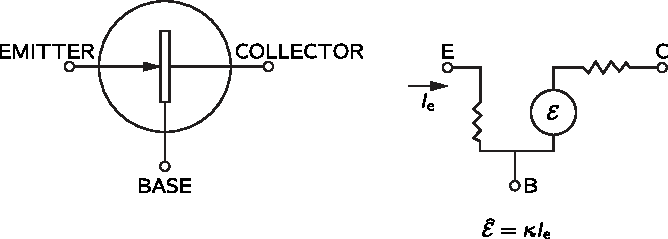
\includegraphics[width=0.9\linewidth]{fyz_fig378.pdf}
    \caption{Ekvivalentní obvod tranzistoru při nízkých frekvencích
             (\cite[s.~415]{Feynman02})}
    \label{fyz:fig378}
  \end{figure}
  
  Naše reprezentace bude muset - podobně jako v případu vzájemné indukčnosti - zahrnovat pomocné 
  generátory napětí, jimiž se popíše vliv napětí nebo proudů v jedné části zařízení na proudy a 
  napětí v jiné jeho části. Například anodový obvod triody lze obvykle reprezentovat jako odpor 
  zapojený do série s ideálním generátorem napětí, jehož emn je přímo úměrné mřížkovému napětí. 
  Dostáváme tak ekvivalentní obvod nakreslený na obr. \ref{fyz:fig377}\footnote{Tento ekvivalentní 
  obvod je správný pouze pro nízké frekvence. Při vysokých frekvencích se ekvivalentní obvod stává 
  složitějším a bude obsahovat různé tzv. parazitní kapacity a indukčnosti.} Podobně kolektorový 
  obvod tranzistoru lze vhodně reprezentovat jako rezistor zapojený do série s ideálním generátorem 
  napětí, jehož velikost je přímo úměrná proudu z emitoru do báze tranzistoru. Ekvivalentní
  obvod pak vypadá tak, jak je nakresleno na obr. \ref{fyz:fig378}. Pro elektronky nebo tranzistory 
  můžeme takové reprezentace používat tehdy, když rovnice popisující jejich činnost jsou lineární. 
  Včlení-li se tato zařízení do složité sítě, zůstávají naše obecné závěry o ekvivalentní 
  reprezentaci libovolného zapojení prvků stále platná. Existuje jedna pozoruhodná věc, kterou se 
  obvody s tranzistory a elektronkami liší od obvodů obsahujících pouze impedance - v nich se totiž 
  reálná část efektivní impedance \(Z\) může stát \emph{zápornou}. Viděli jsme, že reálná část 
  \(Z\) představuje ztrátu energie. Ale důležitou vlastností tranzistorů a elektronek je, že 
  \emph{dodávají} energii do obvodu. (Přirozeně, oni sami „energii“ nevyrábějí, ale odebírají ji ze 
  stejnosměrných obvodů zahrnujících i zdroje napětí a transformují ji na energii střídavého 
  proudu.) Tak je tedy možné dostat obvod se záporným odporem. Takový obvod má tu vlastnost, že 
  když jej připojíme k nějaké impedanci s kladnou reálnou částí, tj. kladné rezistanci, a 
  uspořádáme vše tak, aby součet obou reálných částí byl přesně roven nule, nebude v tomto složeném 
  obvodu docházet ke ztrátám energie. A když žádné ztráty energie nejsou, každé střídavé napětí, 
  které jednou vzniklo, zůstane navždy. To je základní myšlenka, na níž je založena činnost 
  oscilátoru anebo signálového generátoru, kterého lze použít jako zdroj střídavého napětí každé 
  požadované frekvence.
} %tikzset
%~~~~~~~~~~~~~~~~~~~~~~~~~~~~~~~~~~~~~~~~~~~~~~~~~~~~~~~~~~~~~~~~~~~~~~~~~~~~~~~~~~~~~~~~~~~~~~~~~~
\printbibliography[title={Seznam literatury}, heading=subbibliography]
\addcontentsline{toc}{section}{Seznam literatury}